%\documentclass[xcolor=dvipsnames,9pt]{beamer} 
%% 1. DUAL-DISPLAY NOTES:
%\documentclass[hyperref={bookmarks=false}]{beamer}
%\usepackage{pgfpages}
%\setbeameroption{show notes on second screen=left}

% 2. NOTES ON SEPARATE SLIDES:
%\documentclass[xcolor=dvipsnames,9pt,show notes]{beamer}

% 3. NOTES ONLY:
%\documentclass[xcolor=dvipsnames,9pt,show only notes]{beamer}

% 4. HANDOUTS:
%\documentclass[xcolor=dvipsnames,9pt,handout,show notes]{beamer}

% 5. NO NOTES: ONLY ONE THAT BUILDS WITHOUT WARNINGS
\documentclass[xcolor=dvipsnames,9pt,hide notes, mathserif]{beamer}

%\setbeameroption{show only notes}
%\setbeameroption{show notes}

\usepackage{enumerate,amsmath,amssymb,fancyhdr,mathrsfs,amsthm,url,stmaryrd}
\usepackage{pgfpages}
\usepackage{listings}
%\usepackage{enumitem}

%% For creating a handout:
%\pgfpagesuselayout{4 on 1}[border shrink=5mm]
%\mode<handout>{\setbeamercolor{background canvas}{bg=black!5}}


\setbeamerfont{structure}{family=\rmfamily,shape=\scshape} 
\usepackage{graphicx}
\usepackage{tikz}
\usepackage{color}
\usepackage{scalefnt}
\usetikzlibrary{matrix,arrows}

\usepackage{mathrsfs,textcomp}
\setbeamertemplate{navigation symbols}{}
\usepackage{verbatim}
\usepackage[mathcal]{euscript}

% \definecolor{MyDarkBlue}{rgb}{0.2,0.2,0.7}
% \definecolor{Crimson}{rgb}{0.800,0.000,0.200}
 \definecolor{darkred}{rgb}{0.5,0,0}
\definecolor{olivegreen}{cmyk}{0.64,0,0.95,0.40} % PANTONE 582
\setbeamercolor{alerted text}{fg=\ConfColor}

\usecolortheme[named=\ConfColor]{structure} 
\setbeamertemplate{items}[ball] 
\setbeamertemplate{blocks}[rounded][shadow=true] 

%%%% INSERT MACROS %%%%

%\mode<presentation>{\usetheme{boxes}}
%\mode<presentation>{\usetheme{Madrid}}
%boxes,Pittsburgh JuanLesPins, PaloAlto, Singapore, Szeged, Warsaw, Boadilla
%\usetheme{Madrid}
%\usetheme{boxes}  %boxes,Pittsburgh JuanLesPins, PaloAlto, Singapore, Szeged, Warsaw, Boadilla

\usepackage[english]{babel}
\usepackage[latin1]{inputenc}
\usepackage{times}
\usepackage[T1]{fontenc}
% Or whatever. Note that the encoding and the font should match. If T1
% does not look nice, try deleting the line with the fontenc.



%%%%%%%%%%%%% \newcommand{\PUTIN}{{\text {\bf **********PUT IN**********}}}



%\newcommand{\typo}[1]{{\color{red} #1}}
\newcommand{\typo}[1]{{#1}}

\DeclareMathOperator{\dom}{dom}

\newcommand{\todo}[1]{
\ifthenelse{\boolean{todos}}{~\\{\bf TODO(wjd):} \emph{#1}\\}{}
}

% names
\newcommand{\Jiri}{Ji\v{r}\'i}
\newcommand{\Tuma}{T\r{u}ma}
\newcommand{\Palfy}{P\'alfy}
\newcommand{\Pudlak}{Pudl\'ak}
\newcommand{\PP}{P\'alfy-Pudl\'ak}
\newcommand{\PhP}{P\'alfy-Pudl\'ak}
\newcommand{\PAP}{P\'alfy\ and Pudl\'ak}
\newcommand{\Gratzer}{Gr\"{a}tzer}
\newcommand{\<}{\ensuremath{\langle}}
\renewcommand{\>}{\ensuremath{\rangle}}
\newcommand{\beps}{\ensuremath{\boldsymbol{\varepsilon}}}

% SET THEORY & RELATIONS
% To specifiy that the symbol R is a binary relation use: x \rel{R} y
\newcommand{\rel}[1]{\ensuremath{\mathbin{#1}}}
\newcommand{\rR}{\ensuremath{\rel{R}}}  % or just x \rR y
\newcommand{\fld}{\ensuremath{\mathrm{fld}\,}}   % the field of a relation
\newcommand{\ran}{\ensuremath{\mathrm{ran}\,}}   % the range of a relation
\newcommand{\card}{\ensuremath{\mathrm{card}\,}} % cardinality
\newcommand{\res}{\ensuremath{\upharpoonright}}  % restriction
\newcommand{\es}{\ensuremath{\emptyset}}
\newcommand{\lb}{\ensuremath{\llbracket}}
\newcommand{\rb}{\ensuremath{\rrbracket}}
\newcommand{\arity}{\ensuremath{\mathfrak{a}}}
\newcommand{\ar}{\ensuremath{\mathrm{ar}}}

% binary operations
%% \newcommand{\subnormal}{\ensuremath{\trianglelefteqslant}}
%% \newcommand{\supnormal}{\ensuremath{\trianglerighteqslant}}
%% \newcommand{\notsubnormal}{\ensuremath{\ntrianglelefteqslant}}
\renewcommand{\leq}{\ensuremath{\leqslant}}
\renewcommand{\nleq}{\ensuremath{\nleqslant}}
\renewcommand{\geq}{\ensuremath{\geqslant}}
%\renewcommand{\lneq}{\ensuremath{\lneqslant}}
\renewcommand{\gneq}{\ensuremath{\gneqslant}}
\renewcommand{\ngeq}{\ensuremath{\ngeqslant}}
\newcommand{\ssubnormal}{\ensuremath{\vartriangleleft}}
\newcommand{\subnormal}{\ensuremath{\trianglelefteqslant}}
\newcommand{\supnormal}{\ensuremath{\trianglerighteqslant}}
\newcommand{\notsubnormal}{\ensuremath{\ntrianglelefteqslant}}
\newcommand{\meet}{\ensuremath{\wedge}}
\newcommand{\join}{\ensuremath{\vee}}
\newcommand{\Meet}{\ensuremath{\bigwedge}}
\renewcommand{\Join}{\ensuremath{\bigvee}}

% ALGEBRAS

% fields
\newcommand{\F}{\ensuremath{\mathbb{F}}}   % arbitrary field
\newcommand{\Z}{\ensuremath{\mathbb{Z}}}   % integers
\newcommand{\Q}{\ensuremath{\mathbb{Q}}}   % rational numbers
\newcommand{\N}{\ensuremath{\mathbb{N}}}   % natural numbers

\newcommand{\Hom}{\ensuremath{\mathrm{Hom}}}
\newcommand{\HomR}{\ensuremath{\mathrm{Hom}_R}}
\newcommand{\End}{\ensuremath{\mathrm{End}}}
\newcommand{\Aut}{\ensuremath{\mathrm{Aut}}}

\newcommand{\ID}[1]{\ensuremath{\mathcal{ID}(#1)}}
%\newcommand{\idemdec}{\ensuremath{\mbox{Idemdec}(X)}}
\newcommand{\idemdec}{\ID{X}}
\newcommand{\EqX}{\ensuremath{\mbox{Eq}(X)}}
\newcommand{\Eq}{\ensuremath{\mathrm{Eq}}}
\newcommand{\bEq}{\ensuremath{\mathbf{Eq}}}
\newcommand{\bEqX}{\ensuremath{\mathbf{Eq}(X)}}
\newcommand{\Cg}{\ensuremath{\mathrm{Cg}}}
\newcommand{\Sg}{\ensuremath{\mathrm{Sg}}}
\newcommand{\Stab}{\ensuremath{\mathrm{Stab}}}
\newcommand{\bCon}{\ensuremath{\mathbf{Con\,}}}
\newcommand{\Con}{\ensuremath{\mathrm{Con\,}}}
\newcommand{\Sub}{\ensuremath{\mathrm{Sub}}}
\newcommand{\CSub}{\ensuremath{\mathrm{CSub\,}}}
\newcommand{\Pol}{\ensuremath{\mathrm{Pol}}}
\newcommand{\Clo}{\ensuremath{\mathrm{Clo}}}
%\newcommand{\Pol1}{\ensuremath{\mathrm{Pol}_1}}
\newcommand{\Sym}{\ensuremath{\mathrm{Sym}}}
\newcommand{\core}{\ensuremath{\mathrm{core}}}

\newcommand{\ps}[1]{\ensuremath{^{(#1)}}}
\newcommand{\piB}{\ensuremath{\pi_B}}
\newcommand{\hpsi}{\ensuremath{\hat{\psi}}}
\newcommand{\htheta}{\ensuremath{\hat{\theta}}}
%\newcommand{\supi}{\ensuremath{^{(i)}}}
\newcommand{\supi}{\ensuremath{^{i}}}
%\newcommand{\supj}{\ensuremath{^{(j)}}}
\newcommand{\supj}{\ensuremath{^{j}}}

\newcommand{\FLRP}{{\small FLRP}}
\newcommand{\flrp}{{\small FLRP}}

% SOFTWARE
\newcommand{\GAP}{\textsf{GAP}}
\newcommand{\gap}{\textsf{GAP}}
\newcommand{\XGAP}{\textsf{XGAP}}
\newcommand{\xgap}{\textsf{XGAP}}
\newcommand{\uacalc}{\textsf{UACalc}}
\newcommand{\codesize}{\footnotesize}

\newcommand{\tensor}{\ensuremath{\otimes}}

% \newcommand{\ex}{\marginpar[{\LARGE \Bicycle}]{{\LARGE \Bicycle}}}
\newcommand{\leftsubR}{\ensuremath{ { _R }}}
\newcommand{\power}[1]{\ensuremath{\mathscr{P}(#1)}}
\newcommand{\0}{\ensuremath{\mathbf{0}}}
\newcommand{\1}{\ensuremath{\mathbf{1}}}
\newcommand{\2}{\ensuremath{\mathbf{2}}}
\newcommand{\3}{\ensuremath{\mathbf{3}}}
\newcommand{\4}{\ensuremath{\mathbf{4}}}
\newcommand{\5}{\ensuremath{\mathbf{5}}}

\newcommand{\bA}{\ensuremath{\mathbf{A}}}
\newcommand{\cA}{\ensuremath{\mathcal{A}}}
\newcommand{\fA}{\ensuremath{\mathfrak{A}}}
\newcommand{\sA}{\ensuremath{\mathscr{A}}}

\newcommand{\cB}{\ensuremath{\mathcal{B}}}
\newcommand{\bB}{\ensuremath{\mathbf{B}}}
\newcommand{\bBi}{\ensuremath{\mathbf{B}_i}}
\newcommand{\sB}{\ensuremath{\mathscr{B}}}
\newcommand{\fB}{\ensuremath{\mathfrak{B}}}

\newcommand{\bC}{\ensuremath{\mathbf{C}}}
\newcommand{\cC}{\ensuremath{\mathcal{C}}}
\newcommand{\fC}{\ensuremath{\mathfrak{C}}}
\newcommand{\sC}{\ensuremath{\mathscr{C}}}

\newcommand{\bd}{\ensuremath{\mathbf{d}}}

\newcommand{\bE}{\ensuremath{\mathbf{E}}}
\newcommand{\sE}{\ensuremath{\mathscr{E}}}

\newcommand{\bF}{\ensuremath{\mathbf{F}}}
\newcommand{\sF}{\ensuremath{\mathscr{F}}}

\newcommand{\bG}{\ensuremath{\mathbf{G}}}
\newcommand{\sG}{\ensuremath{\mathscr{G}}}
\newcommand{\barG}{\ensuremath{\overline{G}}}
\newcommand{\barg}{\ensuremath{\overline{g}}}
\newcommand{\G}{\ensuremath{\mathfrak{G}}}

\newcommand{\bH}{\ensuremath{\mathbf{H}}}
\newcommand{\sH}{\ensuremath{\mathscr{H}}}
\newcommand{\barH}{\ensuremath{\overline{H}}}
\newcommand{\barh}{\ensuremath{\overline{h}}}

\newcommand{\cI}{\ensuremath{\mathcal{I}}}
\newcommand{\sI}{\ensuremath{\mathscr{I}}}
\newcommand{\fI}{\ensuremath{\mathfrak{I}}}

\newcommand{\cJ}{\ensuremath{\mathcal{J}}}
\newcommand{\sJ}{\ensuremath{\mathscr{J}}}
\newcommand{\fJ}{\ensuremath{\mathfrak{J}}}

\newcommand{\sK}{\ensuremath{\mathscr{K}}}

\newcommand{\bL}{\ensuremath{\mathbf{L}}}
\newcommand{\sL}{\ensuremath{\mathscr{L}}}

\newcommand{\M}{\ensuremath{\mathbb{M}}}
\newcommand{\bM}{\ensuremath{\mathbf{M}}}
\newcommand{\bN}{\ensuremath{\mathbf{N}}}
\newcommand{\bn}{\ensuremath{\mathbf{n}}}

\newcommand{\bO}{\ensuremath{\mathbf{O}}}
\newcommand{\sO}{\ensuremath{\mathscr{O}}}
\newcommand{\cO}{\ensuremath{\mathcal{O}}}

\newcommand{\bOmega}{\ensuremath{\alg \Omega}}
\newcommand{\ConO}{\ensuremath{\Con \bOmega}}

\newcommand{\bP}{\ensuremath{\mathbf{P}}}
\newcommand{\sP}{\ensuremath{\mathscr{P}}}
\newcommand{\cP}{\ensuremath{\mathcal{P}}}

\newcommand{\bR}{\ensuremath{\mathbf{R}}}

\newcommand{\sS}{\ensuremath{\mathscr{S}}}
\newcommand{\bS}{\ensuremath{\mathbf{S}}}
\newcommand{\bs}{\ensuremath{\mathbf{s}}}
\newcommand{\sT}{\ensuremath{\mathscr{T}}}

\newcommand{\V}{\ensuremath{\mathrm{V}}}
\newcommand{\sV}{\ensuremath{\mathscr{V}}}

\newcommand{\bX}{\ensuremath{\mathbf{X}}}
\newcommand{\bx}{\ensuremath{\mathbf{x}}}
\newcommand{\barx}{\ensuremath{\overline{x}}}

\newcommand{\bY}{\ensuremath{\mathbf{Y}}}
\newcommand{\by}{\ensuremath{\mathbf{y}}}
\newcommand{\bary}{\ensuremath{\overline{y}}}

% miscellaneous
\newcommand{\dotsize}{.8pt}
\newcommand{\giant}{\ensuremath{\mathfrak{Gi}}}
\newcommand{\solvable}{\ensuremath{\mathfrak{S}}}
\newcommand{\si}{\ensuremath{\mathfrak{SI}}}
\renewcommand{\iff}{\ensuremath{\quad \Leftrightarrow \quad}}
\newcommand{\ISLE}{{\small ISLE}}
\newcommand{\Soc}{\ensuremath{\mathrm{Soc}}}
\newcommand{\AGL}{\ensuremath{\mathrm{AGL}}}
\newcommand{\Out}{\ensuremath{\mathrm{Out}}}
\newcommand{\Inn}{\ensuremath{\mathrm{Inn}}}
\newcommand{\stab}[1]{\ensuremath{G_{#1}}}
\newcommand{\Gset}{\ensuremath{G\text{-set}}}
\newcommand{\Gsets}{\ensuremath{G\text{-sets}}}
\newcommand{\Mset}{\ensuremath{M\text{-set}}}
\newcommand{\con}[1]{\op{Con}\;\alg #1}	%% Con A  as a set
%\newcommand{\Con}[1]{\alg{Con}\;\alg #1}	%% Con A  as an lattice
\newcommand{\iso}{\DOTSB\cong}			%% isomorphism
\newcommand{\cov}{\prec}		%% a cover sign
\newcommand{\covs}{\succ}		%% the reverse, "a covers b" sign
\newcommand{\ConA}{\ensuremath{\mathbf{Con}(\mathbf{A})}}
\newcommand{\op}{\operatorname}			%% Should be used for J(w) etc.
\newcommand{\alg}[1]{\mathbf{#1}}
\newcommand{\la}{\langle}	     %% left angle for order sequences <a,b>
\newcommand{\ra}{\rangle}	     %% right angle
\newcommand{\id}{\ensuremath{\mathrm{id}}}
\renewcommand{\phi}{\ensuremath{\varphi}}
\newcommand{\bphi}{\ensuremath{\bar{\varphi}}}
\newcommand{\ann}{\ensuremath{\mathrm{ann}}}
\newcommand{\Tor}{\ensuremath{\mathrm{Tor}}}
\newcommand{\image}{\ensuremath{\mathrm{im}}}
\newcommand{\im}{\ensuremath{\mathrm{im}}}
\newcommand{\Tr}{\ensuremath{\mathrm{Tr}}}
\newcommand{\upalpha}{\ensuremath{\alpha^{\uparrow}}}
\newcommand{\downalpha}{\ensuremath{\alpha^{\downarrow}}}
\newcommand{\upbeta}{\ensuremath{\beta^{\uparrow}}}
\newcommand{\downbeta}{\ensuremath{\beta^{\downarrow}}}
\newcommand{\resB}{\ensuremath{|_{_B}}}
\newcommand{\resBi}{\ensuremath{|_{_{B_i}}}}
\newcommand{\eps}{\ensuremath{\varepsilon}}
\newcommand{\hatmap}{\ensuremath{\widehat{\phantom{x}}}}
\newcommand{\one}{\ensuremath{\mathbf{1}}}
\newcommand{\two}{\ensuremath{\mathbf{2}}}
\newcommand{\three}{\ensuremath{\mathbf{3}}}
\newcommand{\tbeta}{\ensuremath{\widetilde{\beta}}}
\newcommand{\hbeta}{\ensuremath{\widehat{\beta}}}
\newcommand{\cick}{\ensuremath{\sC_i}}
\newcommand{\CE}{\ensuremath{\sC_i^{\sE}}}
\newcommand{\CO}{\ensuremath{\sC_i^{\sO}}}
\newcommand{\CICK}{\ensuremath{c_i/\beta \cup c^{K+1}_i/\beta^{\bB_{K+1}}}}
\newcommand{\GL}{\ensuremath{\mathrm{GL}}}
\newcommand{\PSL}{\ensuremath{\mathrm{PSL}}}



\renewcommand{\phi}{\ensuremath{\varphi}}
\newcommand{\Hawaii}{Hawai\kern.05em`\kern.05em\relax i}
\newcommand{\Manoa}{M\=anoa}
%% \newcommand{\GAP}{{\small GAP}}
%% \newcommand{\cd}{\ensuremath{\otimes}}
%% \newcommand{\con}[1]{\ensuremath{\langle #1 \rangle}}
%% \newcommand{\ii}[1]{{\it #1}}
%% \newcommand{\power}[1]{\ensuremath{\mathscr{P}(#1)}}
%% \newcommand{\scrA}{\ensuremath{\mathscr{A}}}
%% \newcommand{\bM}{\ensuremath{\mathbf{M}}}
%% \newcommand{\Mn}{\ensuremath{\mathbf{M}_n}}
%% \newcommand{\bF}{\ensuremath{\mathbf{F}}}
%% \newcommand{\bE}{\ensuremath{\mathbf{E}}}
%% \newcommand{\bR}{\ensuremath{\mathbf{R}}}
%% \newcommand{\bA}{\ensuremath{\mathbf{A}}}
%% \newcommand{\bG}{\ensuremath{\mathbf{G}}}
%% \newcommand{\bH}{\ensuremath{\mathbf{H}}}
%% \newcommand{\bK}{\ensuremath{\mathbf{K}}}
%% \newcommand{\bL}{\ensuremath{\mathbf{L}}}
%% \newcommand{\bB}{\ensuremath{\mathbf{B}}}
%% \newcommand{\svert}{\ensuremath{\; \vert \; }}
%% \newcommand{\Z}{\ensuremath{\mathbb{Z}}}
%% \newcommand{\sE}{\ensuremath{\mathcal{E}}}
%% \newcommand{\sO}{\ensuremath{\mathcal{O}}}
%% \newcommand{\sH}{\ensuremath{\mathcal{H}}}
%% \newcommand{\sS}{\ensuremath{\mathcal{S}}}
%% %\newcommand{\sL}{\ensuremath{\mathcal{L}}}
%% \newcommand{\sL}{\ensuremath{\mathscr{L}}}
%% \newcommand{\bN}{\ensuremath{\mathbf{N}}}
%% \newcommand{\bX}{\ensuremath{\mathbf{X}}}
%% \newcommand{\resB}{\ensuremath{|_{_B}}}
%% \newcommand{\eps}{\ensuremath{\varepsilon}}
%% \newcommand{\sA}{\ensuremath{\mathcal{A}}}
%% \newcommand{\sB}{\ensuremath{\mathcal{B}}}
%% \newcommand{\sC}{\ensuremath{\mathcal{C}}}
%% \newcommand{\SSS}{\text{\emphslb{S}}}
%% \newcommand{\id}{\mbox{id}}
%% \newcommand{\Hom}{\mbox{Hom}}
%% \newcommand{\End}{\ensuremath{\mathrm{End}}}
%% \newcommand{\bEnd}{\ensuremath{\mathbf{End}}}
%% \newcommand{\Aut}{\ensuremath{\mathrm{Aut}}}
%% \newcommand{\bAut}{\ensuremath{\mathbf{Aut}}}
%% \newcommand{\Cg}{\ensuremath{\mathrm{Cg}}}
%% \newcommand{\core}{\ensuremath{\mathrm{core}}}
%% \newcommand{\Con}{\ensuremath{\mathrm{Con}\,}}
%% \newcommand{\bCon}{\ensuremath{\mathbf{Con}\,}}
%% \newcommand{\Sub}{\mbox{Sub}}
%% \newcommand{\bSub}{\ensuremath{\mathbf{Sub}}}
%% \newcommand{\CSub}[1]{\ensuremath{\mathbf{CSub}[#1]}}
%% \newcommand{\csub}{\ensuremath{\mbox{CSub}}}
%% \newcommand{\Stab}{\mbox{Stab}}
%% \newcommand{\bStab}{\ensuremath{\mathbf{Stab}}}
%% \newcommand{\X}{\ensuremath{\mathbf{X}}}
%% \newcommand{\image}{\mbox{im}}
%% \newcommand{\Eq}{\mbox{Eq}}
%% \newcommand{\bEq}{\ensuremath{\mathbf{Eq}}}
%% \newcommand{\bEqX}{\ensuremath{\mathbf{Eq}(X)}}
%% \newcommand{\idemdec}{\ensuremath{\mbox{Idemdec}(X)}}
%% \newcommand{\EqX}{\ensuremath{\mbox{Eq}(X)}}
%% \newcommand{\upalpha}{\ensuremath{\alpha^{\uparrow}}}
%% \newcommand{\downalpha}{\ensuremath{\alpha^{\downarrow}}}
%% \newcommand{\upbeta}{\ensuremath{\beta^{\uparrow}}}
%% \newcommand{\downbeta}{\ensuremath{\beta^{\downarrow}}}
%% \newcommand{\meet}{\ensuremath{\wedge}}
%% \newcommand{\join}{\ensuremath{\vee}}
%% \newcommand{\Meet}{\ensuremath{\bigwedge}}
%% \renewcommand{\Join}{\ensuremath{\bigvee}}
%% \renewcommand{\leq}{\ensuremath{\leqslant}}
%% \renewcommand{\nleq}{\ensuremath{\nleqslant}}
%% \renewcommand{\geq}{\ensuremath{\geqslant}}
 \newcommand{\pb}{\ensuremath{\protect{|}}}

%% % binary operations
%% %% \newcommand{\subnormal}{\ensuremath{\trianglelefteqslant}}
%% %% \newcommand{\supnormal}{\ensuremath{\trianglerighteqslant}}
%% %% \newcommand{\notsubnormal}{\ensuremath{\ntrianglelefteqslant}}
%% %\renewcommand{\lneq}{\ensuremath{\lneqslant}}
%% \newcommand{\ssubnormal}{\ensuremath{\vartriangleleft}}
%% \newcommand{\subnormal}{\ensuremath{\trianglelefteqslant}}
%% \newcommand{\supnormal}{\ensuremath{\trianglerighteqslant}}
%% \newcommand{\notsubnormal}{\ensuremath{\ntrianglelefteqslant}}
%% % \renewcommand{\gneq}{\ensuremath{\gneqslant}}
%% % \renewcommand{\ngeq}{\ensuremath{\ngeqslant}}
%% % \renewcommand{\leq}{\ensuremath{\leqslant}}
%% % \renewcommand{\nleq}{\ensuremath{\nleqslant}}
%% % \renewcommand{\geq}{\ensuremath{\geqslant}}



%% \newcommand{\code}[1]{{\small {\tt #1}}}
%% \newcommand{\<}{\langle}	     %% left angle for order sequences <a,b>
%% \renewcommand{\>}{\rangle}	     %% right angle

%% \newcommand{\Palfy}{P\'alfy}
%% \newcommand{\Pudlak}{Pudl\'ak}
%% \newcommand{\PAP}{P\'alfy-Pudl\'ak}


%% \newcommand{\sI}{\ensuremath{\mathcal{I}}}
%% \newcommand{\hbeta}{\ensuremath{\widehat{\beta}}}
%% \newcommand{\htheta}{\ensuremath{\widehat{\theta}}}
%% \newcommand{\one}{\ensuremath{\mathbf{1}}}
%% \newcommand{\two}{\ensuremath{\mathbf{2}}}
%% \newcommand{\hatmap}{\ensuremath{\widehat{\phantom{x}}}}
%% \newcommand{\Pol}{\ensuremath{\mathrm{Pol}}}
  %%%%%%%%%%%%%%%%%%

\DeclareMathOperator{\dom}{dom}

\newcommand{\todo}[1]{
\ifthenelse{\boolean{todos}}{~\\{\bf TODO(wjd):} \emph{#1}\\}{}
}

% names
\newcommand{\Jiri}{Ji\v{r}\'i}
\newcommand{\Tuma}{T\r{u}ma}
\newcommand{\Palfy}{P\'alfy}
\newcommand{\Pudlak}{Pudl\'ak}
\newcommand{\PP}{P\'alfy-Pudl\'ak}
\newcommand{\PhP}{P\'alfy-Pudl\'ak}
\newcommand{\PAP}{P\'alfy\ and Pudl\'ak}
\newcommand{\Gratzer}{Gr\"{a}tzer}
\newcommand{\<}{\ensuremath{\langle}}
\renewcommand{\>}{\ensuremath{\rangle}}
\newcommand{\beps}{\ensuremath{\boldsymbol{\varepsilon}}}

% SET THEORY & RELATIONS
% To specifiy that the symbol R is a binary relation use: x \rel{R} y
\newcommand{\rel}[1]{\ensuremath{\mathbin{#1}}}
\newcommand{\rR}{\ensuremath{\rel{R}}}  % or just x \rR y
\newcommand{\fld}{\ensuremath{\mathrm{fld}\,}}   % the field of a relation
\newcommand{\ran}{\ensuremath{\mathrm{ran}\,}}   % the range of a relation
\newcommand{\card}{\ensuremath{\mathrm{card}\,}} % cardinality
\newcommand{\res}{\ensuremath{\upharpoonright}}  % restriction
\newcommand{\es}{\ensuremath{\emptyset}}
\newcommand{\lb}{\ensuremath{\llbracket}}
\newcommand{\rb}{\ensuremath{\rrbracket}}
\newcommand{\arity}{\ensuremath{\mathfrak{a}}}
\newcommand{\ar}{\ensuremath{\mathrm{ar}}}

% binary operations
%% \newcommand{\subnormal}{\ensuremath{\trianglelefteqslant}}
%% \newcommand{\supnormal}{\ensuremath{\trianglerighteqslant}}
%% \newcommand{\notsubnormal}{\ensuremath{\ntrianglelefteqslant}}
\renewcommand{\leq}{\ensuremath{\leqslant}}
\renewcommand{\nleq}{\ensuremath{\nleqslant}}
\renewcommand{\geq}{\ensuremath{\geqslant}}
%\renewcommand{\lneq}{\ensuremath{\lneqslant}}
\renewcommand{\gneq}{\ensuremath{\gneqslant}}
\renewcommand{\ngeq}{\ensuremath{\ngeqslant}}
\newcommand{\ssubnormal}{\ensuremath{\vartriangleleft}}
\newcommand{\subnormal}{\ensuremath{\trianglelefteqslant}}
\newcommand{\supnormal}{\ensuremath{\trianglerighteqslant}}
\newcommand{\notsubnormal}{\ensuremath{\ntrianglelefteqslant}}
\newcommand{\meet}{\ensuremath{\wedge}}
\newcommand{\join}{\ensuremath{\vee}}
\newcommand{\Meet}{\ensuremath{\bigwedge}}
\renewcommand{\Join}{\ensuremath{\bigvee}}

% ALGEBRAS

% fields
\newcommand{\F}{\ensuremath{\mathbb{F}}}   % arbitrary field
\newcommand{\Z}{\ensuremath{\mathbb{Z}}}   % integers
\newcommand{\Q}{\ensuremath{\mathbb{Q}}}   % rational numbers
\newcommand{\N}{\ensuremath{\mathbb{N}}}   % natural numbers

\newcommand{\Hom}{\ensuremath{\mathrm{Hom}}}
\newcommand{\HomR}{\ensuremath{\mathrm{Hom}_R}}
\newcommand{\End}{\ensuremath{\mathrm{End}}}
\newcommand{\Aut}{\ensuremath{\mathrm{Aut}}}

\newcommand{\ID}[1]{\ensuremath{\mathcal{ID}(#1)}}
%\newcommand{\idemdec}{\ensuremath{\mbox{Idemdec}(X)}}
\newcommand{\idemdec}{\ID{X}}
\newcommand{\EqX}{\ensuremath{\mbox{Eq}(X)}}
\newcommand{\Eq}{\ensuremath{\mathrm{Eq}}}
\newcommand{\bEq}{\ensuremath{\mathbf{Eq}}}
\newcommand{\bEqX}{\ensuremath{\mathbf{Eq}(X)}}
\newcommand{\Cg}{\ensuremath{\mathrm{Cg}}}
\newcommand{\Sg}{\ensuremath{\mathrm{Sg}}}
\newcommand{\Stab}{\ensuremath{\mathrm{Stab}}}
\newcommand{\bCon}{\ensuremath{\mathbf{Con\,}}}
\newcommand{\Con}{\ensuremath{\mathrm{Con\,}}}
\newcommand{\Sub}{\ensuremath{\mathrm{Sub}}}
\newcommand{\CSub}{\ensuremath{\mathrm{CSub\,}}}
\newcommand{\Pol}{\ensuremath{\mathrm{Pol}}}
\newcommand{\Clo}{\ensuremath{\mathrm{Clo}}}
%\newcommand{\Pol1}{\ensuremath{\mathrm{Pol}_1}}
\newcommand{\Sym}{\ensuremath{\mathrm{Sym}}}
\newcommand{\core}{\ensuremath{\mathrm{core}}}

\newcommand{\ps}[1]{\ensuremath{^{(#1)}}}
\newcommand{\piB}{\ensuremath{\pi_B}}
\newcommand{\hpsi}{\ensuremath{\hat{\psi}}}
\newcommand{\htheta}{\ensuremath{\hat{\theta}}}
%\newcommand{\supi}{\ensuremath{^{(i)}}}
\newcommand{\supi}{\ensuremath{^{i}}}
%\newcommand{\supj}{\ensuremath{^{(j)}}}
\newcommand{\supj}{\ensuremath{^{j}}}

\newcommand{\FLRP}{{\small FLRP}}
\newcommand{\flrp}{{\small FLRP}}

% SOFTWARE
\newcommand{\GAP}{\textsf{GAP}}
\newcommand{\gap}{\textsf{GAP}}
\newcommand{\XGAP}{\textsf{XGAP}}
\newcommand{\xgap}{\textsf{XGAP}}
\newcommand{\uacalc}{\textsf{UACalc}}
\newcommand{\codesize}{\footnotesize}

\newcommand{\tensor}{\ensuremath{\otimes}}

% \newcommand{\ex}{\marginpar[{\LARGE \Bicycle}]{{\LARGE \Bicycle}}}
\newcommand{\leftsubR}{\ensuremath{ { _R }}}
\newcommand{\power}[1]{\ensuremath{\mathscr{P}(#1)}}
\newcommand{\0}{\ensuremath{\mathbf{0}}}
\newcommand{\1}{\ensuremath{\mathbf{1}}}
\newcommand{\2}{\ensuremath{\mathbf{2}}}
\newcommand{\3}{\ensuremath{\mathbf{3}}}
\newcommand{\4}{\ensuremath{\mathbf{4}}}
\newcommand{\5}{\ensuremath{\mathbf{5}}}

\newcommand{\bA}{\ensuremath{\mathbf{A}}}
\newcommand{\cA}{\ensuremath{\mathcal{A}}}
\newcommand{\fA}{\ensuremath{\mathfrak{A}}}
\newcommand{\sA}{\ensuremath{\mathscr{A}}}

\newcommand{\cB}{\ensuremath{\mathcal{B}}}
\newcommand{\bB}{\ensuremath{\mathbf{B}}}
\newcommand{\bBi}{\ensuremath{\mathbf{B}_i}}
\newcommand{\sB}{\ensuremath{\mathscr{B}}}
\newcommand{\fB}{\ensuremath{\mathfrak{B}}}

\newcommand{\bC}{\ensuremath{\mathbf{C}}}
\newcommand{\cC}{\ensuremath{\mathcal{C}}}
\newcommand{\fC}{\ensuremath{\mathfrak{C}}}
\newcommand{\sC}{\ensuremath{\mathscr{C}}}

\newcommand{\bd}{\ensuremath{\mathbf{d}}}

\newcommand{\bE}{\ensuremath{\mathbf{E}}}
\newcommand{\sE}{\ensuremath{\mathscr{E}}}

\newcommand{\bF}{\ensuremath{\mathbf{F}}}
\newcommand{\sF}{\ensuremath{\mathscr{F}}}

\newcommand{\bG}{\ensuremath{\mathbf{G}}}
\newcommand{\sG}{\ensuremath{\mathscr{G}}}
\newcommand{\barG}{\ensuremath{\overline{G}}}
\newcommand{\barg}{\ensuremath{\overline{g}}}
\newcommand{\G}{\ensuremath{\mathfrak{G}}}

\newcommand{\bH}{\ensuremath{\mathbf{H}}}
\newcommand{\sH}{\ensuremath{\mathscr{H}}}
\newcommand{\barH}{\ensuremath{\overline{H}}}
\newcommand{\barh}{\ensuremath{\overline{h}}}

\newcommand{\cI}{\ensuremath{\mathcal{I}}}
\newcommand{\sI}{\ensuremath{\mathscr{I}}}
\newcommand{\fI}{\ensuremath{\mathfrak{I}}}

\newcommand{\cJ}{\ensuremath{\mathcal{J}}}
\newcommand{\sJ}{\ensuremath{\mathscr{J}}}
\newcommand{\fJ}{\ensuremath{\mathfrak{J}}}

\newcommand{\sK}{\ensuremath{\mathscr{K}}}

\newcommand{\bL}{\ensuremath{\mathbf{L}}}
\newcommand{\sL}{\ensuremath{\mathscr{L}}}

\newcommand{\M}{\ensuremath{\mathbb{M}}}
\newcommand{\bM}{\ensuremath{\mathbf{M}}}
\newcommand{\bN}{\ensuremath{\mathbf{N}}}
\newcommand{\bn}{\ensuremath{\mathbf{n}}}

\newcommand{\bO}{\ensuremath{\mathbf{O}}}
\newcommand{\sO}{\ensuremath{\mathscr{O}}}
\newcommand{\cO}{\ensuremath{\mathcal{O}}}

\newcommand{\bOmega}{\ensuremath{\alg \Omega}}
\newcommand{\ConO}{\ensuremath{\Con \bOmega}}

\newcommand{\bP}{\ensuremath{\mathbf{P}}}
\newcommand{\sP}{\ensuremath{\mathscr{P}}}
\newcommand{\cP}{\ensuremath{\mathcal{P}}}
%\newcommand{\cP}{\ensuremath{\mathfrak{X}}}

\newcommand{\bR}{\ensuremath{\mathbf{R}}}

\newcommand{\sS}{\ensuremath{\mathscr{S}}}
\newcommand{\bS}{\ensuremath{\mathbf{S}}}
\newcommand{\bs}{\ensuremath{\mathbf{s}}}
\newcommand{\sT}{\ensuremath{\mathscr{T}}}

\newcommand{\V}{\ensuremath{\mathrm{V}}}
\newcommand{\sV}{\ensuremath{\mathscr{V}}}

\newcommand{\bX}{\ensuremath{\mathbf{X}}}
\newcommand{\bx}{\ensuremath{\mathbf{x}}}
\newcommand{\barx}{\ensuremath{\overline{x}}}

\newcommand{\bY}{\ensuremath{\mathbf{Y}}}
\newcommand{\by}{\ensuremath{\mathbf{y}}}
\newcommand{\bary}{\ensuremath{\overline{y}}}

% miscellaneous
\newcommand{\dotsize}{.8pt}
\newcommand{\giant}{\ensuremath{\mathfrak{Gi}}}
\newcommand{\solvable}{\ensuremath{\mathfrak{S}}}
\newcommand{\si}{\ensuremath{\mathfrak{SI}}}
\renewcommand{\iff}{\ensuremath{\quad \Leftrightarrow \quad}}
\newcommand{\ISLE}{{\small ISLE}}
\newcommand{\Soc}{\ensuremath{\mathrm{Soc}}}
\newcommand{\AGL}{\ensuremath{\mathrm{AGL}}}
\newcommand{\Out}{\ensuremath{\mathrm{Out}}}
\newcommand{\Inn}{\ensuremath{\mathrm{Inn}}}
\newcommand{\stab}[1]{\ensuremath{G_{#1}}}
\newcommand{\Gset}{\ensuremath{G\text{-set}}}
\newcommand{\Gsets}{\ensuremath{G\text{-sets}}}
\newcommand{\Mset}{\ensuremath{M\text{-set}}}
\newcommand{\con}[1]{\op{Con}\;\alg #1}	%% Con A  as a set
%\newcommand{\Con}[1]{\alg{Con}\;\alg #1}	%% Con A  as an lattice
\newcommand{\iso}{\DOTSB\cong}			%% isomorphism
\newcommand{\cov}{\prec}		%% a cover sign
\newcommand{\covs}{\succ}		%% the reverse, "a covers b" sign
\newcommand{\ConA}{\ensuremath{\mathbf{Con}(\mathbf{A})}}
\newcommand{\op}{\operatorname}			%% Should be used for J(w) etc.
\newcommand{\alg}[1]{\mathbf{#1}}
\newcommand{\la}{\langle}	     %% left angle for order sequences <a,b>
\newcommand{\ra}{\rangle}	     %% right angle
\newcommand{\id}{\ensuremath{\mathrm{id}}}
\renewcommand{\phi}{\ensuremath{\varphi}}
\newcommand{\bphi}{\ensuremath{\bar{\varphi}}}
\newcommand{\ann}{\ensuremath{\mathrm{ann}}}
\newcommand{\Tor}{\ensuremath{\mathrm{Tor}}}
\newcommand{\image}{\ensuremath{\mathrm{im}}}
\newcommand{\im}{\ensuremath{\mathrm{im}}}
\newcommand{\Tr}{\ensuremath{\mathrm{Tr}}}
\newcommand{\upalpha}{\ensuremath{\alpha^{\uparrow}}}
\newcommand{\downalpha}{\ensuremath{\alpha^{\downarrow}}}
\newcommand{\upbeta}{\ensuremath{\beta^{\uparrow}}}
\newcommand{\downbeta}{\ensuremath{\beta^{\downarrow}}}
\newcommand{\resB}{\ensuremath{|_{_B}}}
\newcommand{\resBi}{\ensuremath{|_{_{B_i}}}}
\newcommand{\eps}{\ensuremath{\varepsilon}}
\newcommand{\hatmap}{\ensuremath{\widehat{\phantom{x}}}}
\newcommand{\one}{\ensuremath{\mathbf{1}}}
\newcommand{\two}{\ensuremath{\mathbf{2}}}
\newcommand{\three}{\ensuremath{\mathbf{3}}}
\newcommand{\tbeta}{\ensuremath{\widetilde{\beta}}}
\newcommand{\hbeta}{\ensuremath{\widehat{\beta}}}
\newcommand{\cick}{\ensuremath{\sC_i}}
\newcommand{\CE}{\ensuremath{\sC_i^{\sE}}}
\newcommand{\CO}{\ensuremath{\sC_i^{\sO}}}
\newcommand{\CICK}{\ensuremath{c_i/\beta \cup c^{K+1}_i/\beta^{\bB_{K+1}}}}
\newcommand{\GL}{\ensuremath{\mathrm{GL}}}
\newcommand{\PSL}{\ensuremath{\mathrm{PSL}}}



\renewcommand{\phi}{\ensuremath{\varphi}}
\newcommand{\Hawaii}{Hawai\kern.05em`\kern.05em\relax i}
\newcommand{\Manoa}{M\=anoa}
 \newcommand{\pb}{\ensuremath{\protect{|}}}

\title[FLRP]{OVERALGEBRAS:\\{\large expansions and extensions of finite algebras}}
\author[William DeMeo]{William DeMeo\\
  {\small \url{williamdemeo@gmail.com}}}
%% \\{\tiny joint work with}\\
%% {\small Ralph Freese, Peter Jipsen, Bill Lampe, J.B. Nation}}
\institute[\url{williamdemeo@gmail}]{%
  {\color{darkred}  {\small Iowa State University}\\
       Algebra \& Combinatorics Seminar}}

\date{22 Feb 2016}

\subject{Universal Algebra; Lattice Theory.}% (optional) inserted into PDF info catalog.

% If you wish to uncover everything in a step-wise fashion, uncomment the following command: 
% \beamerdefaultoverlayspecification{<+->}

\begin{document}
\thicklines

%% As of 20120415 using this line:
%% \includeonlyframes{decompositions,titlepage,problem,classes,milestones,methods,knownresults,filteridealShort,MO,freese,OA,OAcong,OAEx2,PAP1,OAresults,OAextension,Limitations,OAextension2,conclusion,MO,Conclusion,SubgroupLattice,L7,L7second,IdeaOfL7Proof,OSTheorem,FinalConclusions}
\newcommand{\defn}[1]{\alert{#1}}
\setbeamercovered{transparent}

\frame[label=titlepage]{
  \titlepage
  \vskip-3mm
  \begin{columns}
    \begin{column}{0.8\textwidth}
      \begin{center}
        {\small {\it These slides and other resources are available at}}\\[4pt]
        {{\Large \color{darkred} \url{https://github.com/williamdemeo/Talks}}}
      \end{center}
    \end{column}
  \end{columns}
}

% Commands for creating the ROTATING RECTANGLE
% Pass in a number which will be used to calculate the rotation angle.
% Example: Inside a tikzpicture environment, I would call 
%          \foreach \i in {0,...,11} { \eImageOfBZero{\i}  }
\newcommand{\eImageOfBZero}[1]{
  \pgfmathtruncatemacro{\r}{15*#1}
  \foreach \j in {1,2} {
    \draw[rotate around={\r:(-1,0.5)}] (\j -1, 0.5) node {$\j$};
    \pgfmathtruncatemacro{\x}{\j+3}
    \draw[rotate around={\r:(-1,0.5)}] (\j -1, -0.5) node {$\x$};
  }
  \draw[rotate around={\r:(-1,0.5)}] (-1, -0.5) node {$3$};
  \draw[rounded corners, dotted, rotate around={\r:(-1,0.5)}] (-1.5,-1) rectangle (1.5,1);
}

\newcommand{\eImageOfBOne}[1]{
  \pgfmathtruncatemacro{\r}{-15*#1}
  \foreach \j in {0,1,2} {
    \pgfmathtruncatemacro{\x}{10-\j}
    \draw[rotate around={\r:(-1,0.5)}] (\j -3, 1.5) node {$\x$};
  }
  \draw[rotate around={\r:(-1,0.5)}] (-3, .5) node {$7$} (-2, .5) node {$6$};
  \draw[rounded corners, dotted, rotate around={\r:(-1,0.5)}] (-3.5,0) rectangle (-0.5,2);
}

\newcommand{\eImageOfBTwo}[1]{
  \pgfmathtruncatemacro{\r}{15*#1}
  \foreach \j in {0,1,2} {
    \pgfmathtruncatemacro{\x}{15-\j}
    \draw[rotate around={\r:(1,0.5)}] (\j+1,1.5) node {$\x$};
  }
  \draw[rotate around={\r:(1,0.5)}] (3, .5) node {$11$} (2, .5) node {$12$};
  \draw[rounded corners, dotted,rotate around={\r:(1,0.5)}] (3.5,0) rectangle (0.5,2);
}

  \setbeamercovered{opaque}

\begin{frame}[fragile,label=freese,shrink=5]{Contruction of an algebra $\bA$ with $\Con \bA \cong L_9$.}

  \begin{columns}
    \begin{column}{0.2\textwidth}

      \begin{center}
      \begin{tikzpicture}[scale=.7]
                \node (250) at (2.5,0)  [draw, circle, inner sep=\dotsize] {};
        \node (253) at (2.5,3)  [draw, circle, inner sep=\dotsize] {};
        \foreach \i in {1,...,4} 
                 { 
                   \node (\i15) at (\i,1.5)  [draw, circle, inner sep=\dotsize] {};
                   \draw[semithick] (250) to (\i15) to (253);
                 }

        \uncover<2->{
          \draw[font=\footnotesize] 
          (0.7,1.5) node {$\alpha$} (1.7,1.5) node {$\beta$}
          (3.3,1.5) node {$\gamma$} (4.3,1.5) node {$\delta$}
          (2.8,3.15) node {$1_B$} (2.83,-.15) node {$0_B$};
        }
        \visible<1>{
          \draw  (1,0) node {$M_4$};}
        \visible<2->{
          \draw  (1,0) node {$\Con \bB$};}
      \end{tikzpicture}
      \end{center}

\vskip3mm

      \begin{center}
        \begin{tikzpicture}[scale=.7]

                \node (70) at (6.5,0)  [draw, circle, inner sep=\dotsize] {};
      \node (71) at (7,1.5)  [draw, circle, inner sep=\dotsize] {};
      \node (73) at (6.5,3)  [draw, circle, inner sep=\dotsize] {};
      \node (61) at (6,1.5)  [draw, circle, inner sep=\dotsize] {};
      \node (51) at (5,1)  [draw, circle, inner sep=\dotsize] {};
      \node (52) at (5,2)  [draw, circle, inner sep=\dotsize] {};
      \node (81) at (8,1.5)  [draw, circle, inner sep=\dotsize] {};
      \draw[semithick] 
      (70) to (51) to (52) to (73)
      (70) to (61) to (73) 
      (70) to (71) to (73) 
      (70) to (81) to (73);

          \visible<1-3>{\draw  (5,0) node {$L_{9}$};}
          \visible<4->{\draw  (5,0) node {$\Con \bA$};}
          \visible<4->{\draw[font=\footnotesize] (4.7,2) node {$\widehat{\alpha}$} (4.7,1) node {$\alpha^*$};}

        \end{tikzpicture}
      \end{center}

    \end{column}


    \begin{column}{0.75\textwidth}
      \begin{enumerate}[Step 1]
      \item<2-> 
        Take a permutational algebra $\bB = \<B, F\>$ with congruence lattice $\Con\bB \cong M_4$.

        \vskip6pt
        
        \note{There are infinitely many, but apart from those involving 
          $S_3$, $C_3 \times C_3$, and $(C_3 \times C_3) \rtimes C_3$, they are quite
          large.  The next smallest G-set with $M_4$ congruence lattice that we
          know of comes from the group 
          $G = [ ( (C_3 \times C_3) \rtimes C_2 ) \times ( (C_3 \times C_3) \rtimes C_2 ) ] \rtimes C_2$
          acting on right cosets of $H \cong D_8$.  The index in this case is $|G:H| = 81$.
          (In \GAP, {\tt G:=SmallGroup(648,725)}.)}

        {\small
          \uncover<3->{\underline{Example:}
          \vskip4pt
          \begin{itemize}
%          \begin{itemize}[label=$\cdot$]
          \item
            Let $B = \{0, 1, \dots, 5\}$ index the elements of $S_3$ and
            consider the right regular action of $S_3$ on itself.
            \vskip5pt
          \item
            $g_0 = (0,4)(1,3)(2,5)$ and $g_1 = (0,1,2)(3,4,5)$ generate this
            action group, the image of $S_3 \hookrightarrow S_6$.
            \vskip5pt
          \item $\Con \<B , \{g_0, g_1\}\> \cong M_4$ with congruences
            \[
            \hskip-6mm            \alpha = | 0 1 2 | 3 4 5|, \; \beta = | 0 3 | 1 4 | 2 5 |, 
            \gamma = | 0 4|1 5| 2 3| , \; \delta = | 0 5|1 3| 2 4| .
            \]
          \end{itemize}}
        }

        \vskip6pt

\uncover<4->{
\hskip-10mm {\rmfamily {\bf Goal:} \emph{expand $\bB$ to an algebra $\bA$ that has
          $\alpha$ ``doubled'' in $\Con\bA$.}}}

        \vskip10pt

            \item<5-> Since $\alpha = \Cg^\bB(0,2)$, we let $A = B_0 \cup B_1 \cup B_2$ where
              \vskip-8pt
              \begin{align*}
                B_0 &= \{ {\color<5->{blue}0}, 1, {\color<5->{green}2}, 3, 4, 5\} = B\\
                B_1 &= \{{\color<5->{blue}0}, 6, 7, 8, 9, 10\}\\
                B_2 &= \{ 11, 12, {\color<5->{green}2}, 13, 14, 15\}.
              \end{align*}
            \item<6-> Define unary operations $e_0, e_1, e_2,\, s, \,g_0 e_0$, and $g_1 e_0$.
      \end{enumerate}

    \end{column}

  \end{columns}

\end{frame}

\begin{frame}[fragile,label=freese,shrink=5]{Contruction of an algebra $\bA$ with $\Con \bA \cong L_9$.}
  \begin{columns}

    \begin{column}{0.3\textwidth}
      \vskip2mm
      \begin{tikzpicture}[scale=.7]
                \node (250) at (2.5,0)  [draw, circle, inner sep=\dotsize] {};
        \node (253) at (2.5,3)  [draw, circle, inner sep=\dotsize] {};
        \foreach \i in {1,...,4} 
                 { 
                   \node (\i15) at (\i,1.5)  [draw, circle, inner sep=\dotsize] {};
                   \draw[semithick] (250) to (\i15) to (253);
                 }

        \draw[font=\footnotesize] 
        (0.7,1.5) node {$\alpha$} (1.7,1.5) node {$\beta$}
        (3.3,1.5) node {$\gamma$} (4.3,1.5) node {$\delta$}
        (2.8,3.15) node {$1_B$} (2.83,-.15) node {$0_B$};
      \end{tikzpicture}
    \end{column}

    \begin{column}{0.4\textwidth}
      \begin{tikzpicture}[scale=.7]
              \node (70) at (6.5,0)  [draw, circle, inner sep=\dotsize] {};
      \node (71) at (7,1.5)  [draw, circle, inner sep=\dotsize] {};
      \node (73) at (6.5,3)  [draw, circle, inner sep=\dotsize] {};
      \node (61) at (6,1.5)  [draw, circle, inner sep=\dotsize] {};
      \node (51) at (5,1)  [draw, circle, inner sep=\dotsize] {};
      \node (52) at (5,2)  [draw, circle, inner sep=\dotsize] {};
      \node (81) at (8,1.5)  [draw, circle, inner sep=\dotsize] {};
      \draw[semithick] 
      (70) to (51) to (52) to (73)
      (70) to (61) to (73) 
      (70) to (71) to (73) 
      (70) to (81) to (73);

        \draw[font=\footnotesize] 
        (4.7,1) node {$\alpha^*$} (4.7,2) node {$\widehat{\alpha}$}
        (5.7,1.5) node {$\beta^*$} (7.3,1.5) node {$\gamma^*$} (8.3,1.5) node {$\delta^*$}
        (6.8,3.15) node {$1_A$} (6.83,-.15) node {$0_A$};
      \end{tikzpicture}
    \end{column}

  \end{columns}

  \begin{columns}
    \begin{column}{0.3\textwidth}
      \begin{center}
        $\Con \< B,\{g_0, g_1\}\>$

        \vskip-2pt
        \begin{align*}
          \alpha &= {\color<2->{blue}\pb 0, 1, 2 \pb 3, 4, 5\pb }\\[4pt]
          \beta &= {\color<2->{blue}\pb 0, 3 \pb  1, 4 \pb 2, 5 \pb} \\[3pt]
          \gamma &= {\color<2->{blue}\pb 0, 4\pb 1, 5\pb  2, 3\pb}  \\[3pt]
          \delta &= {\color<2->{blue}\pb 0, 5\pb 1, 3\pb  2, 4\pb} 
        \end{align*}
      \end{center}
    \end{column}

    \begin{column}{0.65\textwidth}
      \begin{center}
        $\Con \<A, F_A\>$
      \end{center}
      \begin{align*}
        \widehat{\alpha} &=|{\color<2->{blue}0,1,2},6,7,11,12|{\color<2->{blue}3,4,5}|8,9,10,13,14,15| \\
        \alpha^* &=|{\color<2->{blue}0,1,2},6,7,11,12|{\color<2->{blue}3,4,5}|8,9,10|13,14,15| \\[2pt]
        \beta^*&=|{\color<2->{blue}0,3},8|{\color<2->{blue}1,4}|{\color<2->{blue}2,5},15|6,9|7,10|11,13|12,14| \\[2pt]
        \gamma^*&=|{\color<2->{blue}0,4},9|{\color<2->{blue}1,5}|{\color<2->{blue}2,3},13|6,10|7,8|11,14|12,15| \\[2pt]
        \delta^*&=|{\color<2->{blue}0,5},10|{\color<2->{blue}1,3}|{\color<2->{blue}2,4},14|6,8|7,9,11,15|12,13|
      \end{align*}
    \end{column}
  \end{columns}

  \vskip4mm

  \only<2>{\[
    \alpha = \alpha^*\cap B^2 = \widehat{\alpha}\cap B^2,\; \quad
    \beta = \beta^*\cap B^2, \quad \dots %\quad \gamma = \gamma^*\cap B^2, \quad \delta = \delta^*\cap B^2.
    \]}

\end{frame}

\newcommand{\ifdot}{dotted}
%\newcommand{\ifdot}{dashed}
%\newcommand{\ifdot}{}

\begin{frame}[fragile,label=OA,shrink=5]{Extension \& Expansion}
  \begin{columns}
    \begin{column}{0.3\textwidth}
      \begin{center}
        $\Con \< B,\{g_0, g_1\}\>$

        \vskip-2pt
        \begin{align*}
          \alpha &= |{\color<2,6,7>{blue}0, 1, 2} | {\color<2,6,7>{blue}3, 4, 5}|\\[4pt]
          \beta &= |{\color<3>{blue}0, 3} | {\color<3>{blue}1, 4} |{\color<3>{blue}2, 5} | \\[3pt]
          \gamma &= |{\color<4>{blue}0, 4}|{\color<4>{blue}1, 5}|{\color<4>{blue}2, 3}| \\[3pt]
          \delta &= |{\color<5>{blue}0, 5}|{\color<5>{blue}1, 3}|{\color<5>{blue} 2, 4}| 
        \end{align*}
      \end{center}
    \end{column}

    \begin{column}{0.4\textwidth}
      {
        \begin{tikzpicture}[scale=.7]

          \visible<1-48,62->{ % B_0
            \foreach \j in {0,1,2} {
              \draw (\j -1, 0.5) node {$\j$};
              \pgfmathtruncatemacro{\x}{\j+3}
              \draw (\j -1, -0.5) node {$\x$};
            }
            \draw (0,-1.5) node {$B_0$};
          }

          \visible<2,6>{ % alpha
            \draw[rounded corners,\ifdot] (-1.3,-.8) rectangle (1.3,-.2);
            \draw[rounded corners,\ifdot] (-1.3,.8) rectangle (1.3,.2);
            \draw[font=\Large] (-2,-1) node {$\alpha$};
          }
          \visible<3>{  % beta
            \draw[rounded corners,\ifdot] (-1.3,-.8) rectangle (-.7,.8);
            \draw[rounded corners,\ifdot] (-.3,-.8) rectangle (.3,.8);
            \draw[rounded corners,\ifdot] (1.3,-.8) rectangle (.7,.8);
            \draw[font=\Large] (-2,-1) node {$\beta$};
          }
          \visible<4>{   % beta
            \draw[rounded corners,\ifdot] (1,-.85) to (1.35,-.5) to  (-0,.85) to (-.35,.5) to (1,-.85);
            \draw[rounded corners,\ifdot] (0,-.85) to (0.35,-.5) to  (-1,.85) to (-1.35,.5) to (0,-.85);
            \draw[rounded corners,\ifdot] (.8,.05) to (1.37,.35) to  (1.1,.87) to (.4,.4);
            \draw[rounded corners,\ifdot] (-.8,-.05) to (-1.37,-.35) to  (-1.1,-.87) to (-.4,-.4);
            \draw[\ifdot] (-0.1,.2) to (-.28,.13);
            \draw[\ifdot] (0.1,-.2) to (.28,-.13);
            \draw[font=\Large] (-2,-1) node {$\gamma$};
          }

          \visible<5>{ % delta
            \draw[rounded corners,\ifdot] (-1,-.85) to (-1.35,-.5) to  (0,.85) to (.35,.5) to (-1,-.85);
            \draw[rounded corners,\ifdot] (0,-.85) to (-0.35,-.5) to  (1,.85) to (1.35,.5) to (0,-.85);
            \draw[rounded corners,\ifdot] (-.8,.05) to (-1.37,.35) to  (-1.1,.87) to (-.4,.4);
            \draw[rounded corners,\ifdot] (.8,-.05) to (1.37,-.35) to  (1.1,-.87) to (.4,-.4);
            \draw[\ifdot] (0.1,.2) to (.28,.13);
            \draw[\ifdot] (-0.1,-.2) to (-.28,-.13);
            \draw[font=\Large] (-2,-1) node {$\delta$};
          }

          %% B0 rectangle %%
          \visible<8-34>{\draw[rounded corners,blue] (-1.5,-1) rectangle (1.5,1); }
          \visible<1-7,35-48,62->{\draw[rounded corners,dotted] (-1.5,-1) rectangle (1.5,1);}

          %% B1 %%
          \visible<7,35->{ 
            \foreach \j in {0,1,2} {
              \pgfmathtruncatemacro{\x}{10-\j}
              \draw (\j -3, 1.5) node {$\x$};
            }
            \draw (-3, .5) node {$7$} (-2, .5) node {$6$}; 
          }
          \visible<7,8,35->{\draw  (-2,2.5) node {$B_1$};}
          \visible<7,62->{\draw[rounded corners,dotted] (-3.5,0) rectangle (-0.5,2);}
          \visible<35-61>{\draw[rounded corners,blue] (-3.5,0) rectangle (-0.5,2);}
          \visible<49-61>{\draw (-1, .5) node {$0$}; }

          %% B2 %%
          \visible<7-21,62->{ 
            {\color<9-21>{gray}
              \foreach \j in {0,1,2} {
                \pgfmathtruncatemacro{\y}{15-\j}
                \draw (\j +1, 1.5) node {$\y$};
              }
              \draw (3, .5) node {$11$} (2, .5) node {$12$};
            }
          }
          \visible<7-22,35,62->{\draw  (2,2.5) node {$B_2$};}
          \visible<7-21,62->{\draw[rounded corners,dotted] (3.5,0) rectangle (0.5,2);}

          \foreach \i in {0,...,11}{
            \pgfmathtruncatemacro{\v}{\i+8}
            \visible<\v>{ 
              {\color<18-19>{gray}
                \eImageOfBOne{\i}}
            }
          }
          \foreach \i in {0,...,11}{
            \pgfmathtruncatemacro{\v}{\i+22}
            \visible<\v>{ 
              {\color<32-33>{gray}
                \eImageOfBTwo{\i}
              }
            }
          }

          \foreach \i in {0,...,11}{
            \pgfmathtruncatemacro{\v}{\i+35}
            \visible<\v>{ 
              {\color<46-47>{gray}
                \eImageOfBTwo{\i}
              }
            }
          }

        %% Rotate B0 onto B1 %%
        \foreach \i in {0,1,...,11}{
          \pgfmathtruncatemacro{\v}{\i+49}
          \visible<\v>{ 
            {\color<60-61>{gray}
              \eImageOfBZero{\i}       %% use -\i for clockwise rotation
            }
          }
        }

        \end{tikzpicture}
      }
    \end{column}
  \end{columns}
  \begin{columns}
    \begin{column}{0.3\textwidth}
      \begin{itemize}
      \item<7-> $A = B_0 \cup B_1 \cup B_2$
        \vskip4pt
      \item<8->Unary operations 
        \begin{align*}
          \alt<8-34>{{\color{blue} e_0} & {\color{blue} : A \twoheadrightarrow B_0 }}
                    {{\color{gray} e_0} & {\color{gray} : A \twoheadrightarrow B_0 }}\\
          \alt<35-61>{{\color{blue} e_1} &{\color{blue} : A \twoheadrightarrow B_1}}
                     {{\color{gray} e_1} &{\color{gray} : A \twoheadrightarrow B_1}}\\
          {\color{gray} e_2} &{\color{gray} : A \twoheadrightarrow B_2}\\
          \alt<62>{{\color{blue} s} &{\color{blue} : A \twoheadrightarrow B_0}}
                  {{\color{gray} s} &{\color{gray} : A \twoheadrightarrow B_0}}\\
        \end{align*}
        \[
        \alt<63>{{\color{blue} g e_0} {\color{blue} : A \stackrel{e_0}{\twoheadrightarrow} B_0 \stackrel{g}{\rightarrow} B_0}}
                {{\color{gray} g e_0} {\color{gray} : A \stackrel{e_0}{\twoheadrightarrow} B_0 \stackrel{g}{\rightarrow} B_0}}
        \]
      \end{itemize}
    \end{column}
    \begin{column}{0.5\textwidth}
      \begin{tikzpicture}[scale=.7]

        \visible<6->{                      
          
          %%% B_0 %%%
          \draw (-1,0) node {$B_0 = \{$};
          \foreach \i in { 0, 1, 2, 3, 4, 5}{ 
            \draw (\i,0) node {$\i$}; 
            \visible<8,9,12,13,16,17,20,21-34>{ \draw [|->] (\i,1.1) -- (\i,0.5);}
            \visible<8-23,26-28,31-34>{ \draw [|->] (\i,-1.1) -- (\i,-0.5); }
            \visible<35,49,50,53,54,57,58,60>{ \draw [|->] (\i,0.5) -- (\i,1.1);}
            \visible<35,37,38,41,42,45,46,48>{ \draw [|->] (\i,-1.1) -- (\i,-0.5); }
          }
          \draw (5.5,0) node {$\}$};
        }
        
        \visible<7->{                                               

          %%% B_1 %%%
          \draw (-1,1.5) node {$B_1 =\{$} (0,1.5) node {$0$};
          \foreach \i in { 6, 7, 8, 9, 10}{ \draw (\i-5,1.5) node {$\i$}; }
          \draw (5.5,1.5) node {$\}$};
          
          %%% B_2 %%%
          \draw (-1,-1.5) node {$B_2 =\{$} (0,-1.5) node {$11$} (1,-1.5) node {$12$} (2,-1.5) node {$2$};
          \foreach \i in { 13, 14, 15}{ \draw (\i-10,-1.5) node {$\i$}; }
          \draw (5.5,-1.5) node {$\}$};
        }

      \end{tikzpicture}
    \end{column}

  \end{columns}
\end{frame}





\begin{frame}[fragile,label=OAop3,shrink=5]{Extension \& Expansion}

  \begin{columns}
    \begin{column}{0.3\textwidth}
      \begin{center}
        $\Con \< B,\{g_0, g_1\}\>$

        \vskip-2pt
        \begin{align*}
          \alpha &= |0, 1, 2 | 3, 4, 5|\\[4pt]
          \beta &= |0, 3 | 1, 4 |2, 5 | \\[3pt]
          \gamma &= |0, 4| 1, 5|2, 3| \\[3pt]
          \delta &= |0, 5|1, 3|2, 4| 
        \end{align*}
      \end{center}
    \end{column}

    \begin{column}{0.3\textwidth}
      \begin{tikzpicture}[scale=.7]

        %% B0 %%
        \foreach \j in {0,1,2} {
          \draw (\j -1, 0.5) node {$\j$};
          \pgfmathtruncatemacro{\x}{\j+3}
          \draw (\j -1, -0.5) node {$\x$};
        }
        \draw (0,-1.5) node {$B_0$};
        \draw[rounded corners,dotted] (-1.5,-1) rectangle (1.5,1);

        %% B1 %%
        \foreach \j in {0,1,2} {
          \pgfmathtruncatemacro{\x}{10-\j}
          \draw (\j -3, 1.5) node {$\x$};
        }
        \draw (-3, .5) node {$7$} (-2, .5) node {$6$}; 
        \draw[rounded corners,dotted] (-3.5,0) rectangle (-0.5,2);
        \draw  (-2,2.5) node {$B_1$};

        %% B2 %%
        \foreach \j in {0,1,2} {
          \pgfmathtruncatemacro{\y}{15-\j}
          \draw (\j +1, 1.5) node {$\y$};
        }
        \draw (3, .5) node {$11$} (2, .5) node {$12$};
        \draw  (2,2.5) node {$B_2$};
        \draw[rounded corners,dotted] (3.5,0) rectangle (0.5,2);


      \end{tikzpicture}
    \end{column}
  \end{columns}
  \begin{columns}
    \begin{column}{0.3\textwidth}
      \begin{itemize}
      \item $A = B_0 \cup B_1 \cup B_2$
        \vskip4pt
      \item Unary operations 
        \begin{align*}
          {\color{gray} e_0} & {\color{gray} : A \twoheadrightarrow B_0 } \\
          {\color{gray} e_1} &{\color{gray} : A \twoheadrightarrow B_1}\\
          {\color{gray} e_2} &{\color{gray} : A \twoheadrightarrow B_2}\\
          {\color{blue} s} &{\color{blue} : A \twoheadrightarrow B_0}
        \end{align*}
        \[
          {\color{gray} g e_0} {\color{gray} : A \stackrel{e_0}{\twoheadrightarrow} B_0 \stackrel{g}{\rightarrow} B_0}
          \]
      \end{itemize}
    \end{column}
    \begin{column}{0.5\textwidth}
      \begin{tikzpicture}[scale=.7]

        %%% B_0 %%%
        \draw (-1,0) node {$B_0 = \{$};
        \foreach \i in { 0, 1, 2, 3, 4, 5}{ 
          \draw (\i,0) node {$\i$}; 
        }
        \draw (5.5,0) node {$\}$};

        %%% B_1 %%%
        \draw (-1,1.5) node {$B_1 =\{$} (0,1.5) node {$0$};
        \foreach \i in { 6, 7, 8, 9, 10}{ \draw (\i-5,1.5) node {$\i$}; }
        \draw (5.5,1.5) node {$\}$};
        
        %%% B_2 %%%
        \draw (-1,-1.5) node {$B_2 =\{$} (0,-1.5) node {$11$} (1,-1.5) node {$12$} (2,-1.5) node {$2$};
        \foreach \i in { 13, 14, 15}{ \draw (\i-10,-1.5) node {$\i$}; }
        \draw (5.5,-1.5) node {$\}$};


      \end{tikzpicture}
    \end{column}

  \end{columns}
\end{frame}



\renewcommand{\ifdot}{dotted}
\begin{frame}[fragile,label=OAcong,shrink=5]{Why does it work?}

  \begin{columns}
    \begin{column}{0.3\textwidth}
      \begin{center}
        $\Con \< B,\{g_0, g_1\}\>$

        \vskip-2pt
        \begin{align*}
          \alpha &= {\color<2>{blue} \pb 0, 1, 2 \pb 3, 4, 5\pb }\\[4pt]
          \beta &= {\color<5>{blue} \pb 0, 3 \pb 1, 4 \pb 2, 5 \pb} \\[3pt]
          \gamma &= |0, 4| 1, 5|2, 3| \\[3pt]
          \delta &= |0, 5|1, 3|2, 4| 
        \end{align*}
      \end{center}
    \end{column}

    \begin{column}{0.3\textwidth}
      \begin{tikzpicture}[scale=.7]

        %% B0 %%
        \foreach \j in {0,1,2} {
          \draw (\j -1, 0.5) node {$\j$};
          \pgfmathtruncatemacro{\x}{\j+3}
          \draw (\j -1, -0.5) node {$\x$};
        }
        \draw (0,-1.5) node {$B_0$};
        \draw[rounded corners,dotted] (-1.5,-1) rectangle (1.5,1);

        %% B1 %%
        \foreach \j in {0,1,2} {
          \pgfmathtruncatemacro{\x}{10-\j}
          \draw (\j -3, 1.5) node {$\x$};
        }
        \draw (-3, .5) node {$7$} (-2, .5) node {$6$}; 
        \draw[rounded corners,dotted] (-3.5,0) rectangle (-0.5,2);
        \draw  (-2,2.5) node {$B_1$};

        %% B2 %%
        \foreach \j in {0,1,2} {
          \pgfmathtruncatemacro{\y}{15-\j}
          \draw (\j +1, 1.5) node {$\y$};
        }
        \draw (3, .5) node {$11$} (2, .5) node {$12$};
        \draw  (2,2.5) node {$B_2$};
        \draw[rounded corners,dotted] (3.5,0) rectangle (0.5,2);

        \visible<2>{ % alpha
          \draw[rounded corners,blue] (-1.3,-.8) rectangle (1.3,-.2);
          \draw[rounded corners,blue] (-1.3,.8) rectangle (1.3,.2);
          \draw[font=\Large] (-2,-1) node {$\alpha$};
        }
        \visible<3,4>{ % \alpha^*
          % B0 lower rectangle
          \draw[rounded corners,blue] (-1.3,-.8) rectangle (1.3,-.2);
          % long rectangle
          \draw[rounded corners,blue] (-3.3,.8) rectangle (3.3,.2); 
        }
        \visible<3>{ % \alpha^*
          \draw[rounded corners,blue] (-3.3,1.2) rectangle (-.7,1.8);  
          \draw[rounded corners,blue] (3.3,1.2) rectangle (.7,1.8); 
          \draw[font=\Large] (-2,-1) node {$\alpha^*$};
        }
        \visible<4>{ % \widehat{\alpha}
          \draw[rounded corners,blue] (-3.3,1.2) rectangle (3.3,1.8);  
          \draw[font=\Large] (-2,-1) node {$\widehat{\alpha}$};
        }
        \visible<5>{  % beta
          \draw[rounded corners,blue] (-1.3,-.8) rectangle (-.7,.8);
          \draw[rounded corners,blue] (-.3,-.8) rectangle (.3,.8);
          \draw[rounded corners,blue] (1.3,-.8) rectangle (.7,.8);
          \draw[font=\Large] (-2,-1) node {$\beta$};
        }
        \visible<6->{  % beta
          \draw[rounded corners,blue] (-1.3,-.8) rectangle (-.7,1.85);  % big left rect
          \draw[rounded corners,blue] (-.3,-.8) rectangle (.3,.8);
          \draw[rounded corners,blue] (1.3,-.8) rectangle (.7,1.85);  % big right rect
          \draw[rounded corners,blue] (-1.7,.15) rectangle (-2.3,1.85);
          \draw[rounded corners,blue] (-2.7,.15) rectangle (-3.3,1.85);  % small B1 far left
          \draw[rounded corners,blue] (1.7,.15) rectangle (2.3,1.85);
          \draw[rounded corners,blue] (2.7,.15) rectangle (3.3,1.85); % small B2 far right
          \draw[font=\Large] (-2,-1) node {$\beta^*$};
        }

      \end{tikzpicture}
    \end{column}
  \end{columns}
  \begin{columns}
    \begin{column}{0.3\textwidth}
      \visible<7>{\emph{Why don't the $\beta$ classes of $B_1$ and $B_2$ mix?}}
    \end{column}
    \begin{column}{0.5\textwidth}
      \begin{center}
        $\Con \<A, F_A\>$
      \end{center}
      \begin{align*}
        \widehat{\alpha} &= {\color<4>{blue} \pb 0,1,2,6,7,11,12\pb 3,4,5 \pb 8,9,10,13,14,15\pb } \\
        \alpha^* &= {\color<3>{blue} \pb  0,1,2,6,7,11,12 \pb 3,4,5 \pb 8,9,10 \pb 13,14,15 \pb}  \\[2pt]
        \beta^*&= {\color<6->{blue} \pb 0,3,8 \pb 1,4 \pb 2,5,15 \pb 6,9 \pb 7,10 \pb 11,13 \pb 12,14 \pb } \\[2pt]
        \gamma^*&= \pb 0,4,9 \pb 1,5 \pb 2,3,13 \pb 6,10 \pb 7,8 \pb 11,14 \pb 12,15 \pb  \\[2pt]
        \delta^*&= \pb 0,5,10 \pb 1,3 \pb 2,4,14 \pb 6,8 \pb 7,9,11,15 \pb 12,13 \pb 
      \end{align*}
    \end{column}

  \end{columns}
\end{frame}

\begin{frame}[fragile,label=OAEx2,shrink=5]{Variations on the same example... }

  \begin{columns}
    \begin{column}{0.7\textwidth}
      \begin{itemize}
      \item 
        Suppose we want $\beta = \Cg^\bB(0,3) =| 0, 3 | 2, 5 | 1, 4 |$ to 
        \vskip4pt
        have non-trivial inverse image $\beta\resB^{-1} = [\beta^*, \widehat{\beta}]$.  
        \vskip6pt
      \item<2-> Select elements 0 and 3 as intersection points:
        \[
        A = B_0 \cup B_1 \cup B_2 \quad \text{where}
        \]
        \begin{align*}
          B_0 &= \{{\color{blue} 0}, 1,  2,  {\color{green}3},  4,  5\}\\
          B_1 &= \{{\color{blue} 0}, 6,  7,  8,  9, 10\}\\
          B_2 &= \{11, 12, 13, {\color{green}3}, 14, 15\}.
        \end{align*}
      \end{itemize}
    \end{column}
    \begin{column}{0.3\textwidth}
      \begin{tikzpicture}[scale=.9]
                \node (250) at (2.5,0)  [draw, circle, inner sep=\dotsize] {};
        \node (253) at (2.5,3)  [draw, circle, inner sep=\dotsize] {};
        \foreach \i in {1,...,4} 
                 { 
                   \node (\i15) at (\i,1.5)  [draw, circle, inner sep=\dotsize] {};
                   \draw[semithick] (250) to (\i15) to (253);
                 }

        \draw[font=\small] 
        (0.7,1.5) node {$\alpha$} (1.7,1.5) node {$\beta$}
        (3.3,1.5) node {$\gamma$} (4.3,1.5) node {$\delta$}
        (2.8,3.15) node {$1_B$} (2.83,-.15) node {$0_B$};
      \end{tikzpicture}

    \end{column}

  \end{columns}

  \vskip-5mm

  \begin{columns}
    \begin{column}{0.3\textwidth}

      \begin{tikzpicture}[scale=.8]

        %% B0 %%
        \foreach \j in {0,1,2} {
          \draw (\j -1, 0.5) node {$\j$};
          \pgfmathtruncatemacro{\x}{\j+3}
          \draw (\j -1, -0.5) node {$\x$};
        }
        \draw (1,-1.5) node {$B_0$};
        \draw[rounded corners,dotted] (-1.4,-.9) rectangle (1.4,.9);

        \visible<3->{

          %% B1 %%
          \foreach \j in {0,1,2} {
            \pgfmathtruncatemacro{\x}{10-\j}
            \draw (\j -3, 1.5) node {$\x$};
          }
          \draw (-3, .5) node {$7$} (-2, .5) node {$6$}; 
          \draw[rounded corners,dotted] (-3.5,1.9) rectangle (-0.6,.1);
          \draw  (-4,2) node {$B_1$};

          %% B2 %%
          \foreach \j in {0,1,2} {
            \pgfmathtruncatemacro{\y}{13-\j}
            \draw (\j -3, -1.5) node {$\y$};
          }
          \draw (-3, -.5) node {$15$} (-2, -.5) node {$14$};
          \draw  (-4,-2) node {$B_2$};
          \draw[rounded corners,dotted] (-3.4,-1.9) rectangle (-0.6,-.1);
        }

        \visible<1-3>{  % beta
          \draw[rounded corners,blue] (-1.3,-.8) rectangle (-.7,.8);
          \draw[rounded corners,blue] (-.3,-.8) rectangle (.3,.8);
          \draw[rounded corners,blue] (1.3,-.8) rectangle (.7,.8);
          \draw[font=\Large] (2,0) node {$\beta$};
        }
        \visible<4>{  % beta^*
          \draw[rounded corners,blue] (-1.3,-1.8) rectangle (-.7,1.8);  % big rect
          \draw[rounded corners,blue] (-.3,-.8) rectangle (.3,.8);
          \draw[rounded corners,blue] (.7,-.8) rectangle (1.3,.8);     % right rect
          \draw[rounded corners,blue] (-1.7,.2) rectangle (-2.3,1.8);  % small B1 middle
          \draw[rounded corners,blue] (-2.7,.2) rectangle (-3.3,1.8);  % small B1 left
          \draw[rounded corners,blue] (-1.7,-.2) rectangle (-2.3,-1.8);% small B2 middle 
          \draw[rounded corners,blue] (-2.7,-.2) rectangle (-3.3,-1.8);% small B2 far left
          \draw[font=\Large] (2,0) node {$\beta^*$};
        }
        \visible<5>{  % \widehat{\beta}
          \draw[rounded corners,blue] (-1.3,-1.8) rectangle (-.7,1.8);  % big B0 rect
          \draw[rounded corners,blue] (-.3,-.8) rectangle (.3,.8);        % middle B0 rect
          \draw[rounded corners,blue] (.7,-.8) rectangle (1.3,.8);        % right B0 rect
          \draw[rounded corners,blue] (-3.3,-1.8) rectangle (-2.7,1.8);    % large far left
          \draw[rounded corners,blue] (-2.3,-1.8) rectangle (-1.7,1.8);  % small B2 far left
          \draw[font=\Large] (2,0) node {$\widehat{\beta}$};
        }
        \visible<6>{  % beta\eps1
          \draw[rounded corners,blue] (-1.3,-1.8) rectangle (-.7,1.8); % big rect
          \draw[rounded corners,blue] (-.3,-.8) rectangle (.3,.8);     % middle B0 rect
          \draw[rounded corners,blue] (.7,-.8) rectangle (1.3,.8);     % right rect
          \draw[rounded corners,blue] (-2.7,.2) rectangle (-3.3,1.8);  % small B1 left
          \draw[rounded corners,blue] (-1.7,1.8) rectangle (-2.3,-1.8);% big B1B2 middle 
          \draw[rounded corners,blue] (-2.7,-.2) rectangle (-3.3,-1.8);% small B2 far left
          \draw[font=\Large] (2,0) node {$\beta_\eps$};
        }
        \visible<7->{  % beta\eps2
          \draw[rounded corners,blue] (-1.3,-1.8) rectangle (-.7,1.8); % big rect
          \draw[rounded corners,blue] (-.3,-.8) rectangle (.3,.8);     % middle B0 rect
          \draw[rounded corners,blue] (.7,-.8) rectangle (1.3,.8);     % right rect
          \draw[rounded corners,blue] (-1.7,.2) rectangle (-2.3,1.8);  % small B1 middle
          \draw[rounded corners,blue] (-1.7,-.2) rectangle (-2.3,-1.8);% small B2 middle 
          \draw[rounded corners,blue] (-2.7,1.8) rectangle (-3.3,-1.8);%  big B1/B2 left
          \draw[font=\Large] (2,0) node {$\beta_{\eps'}$};
        }

      \end{tikzpicture}

    \end{column}

    \newcommand{\bigdotsize}{1.5pt}
    \begin{column}{0.3\textwidth}
      \centering
      \visible<4->{
        \begin{tikzpicture}[scale=1]
          \node (bottom) at (6.5,0)  [draw, circle, inner sep=\dotsize] {};  % bottom
          \node (71) at (7,1.5)  [draw, circle, inner sep=\dotsize] {};  % delta
          \node (top) at (6.5,3)  [draw, circle, inner sep=\dotsize] {}; % top
          \alt<4>{\node (61) at (6.1,1)  [fill, circle, red, inner sep=\bigdotsize] {};}  % beta^*}
                 {\node (61) at (6.1,1)  [draw, circle, inner sep=\dotsize] {};}  
                 \alt<5>{\node (62) at (6.1,2)  [fill, circle, red, inner sep=\bigdotsize] {};}  % hat{beta}
                        {\node (62) at (6.1,2)  [draw, circle, inner sep=\dotsize] {};}  % hat{beta}
                        \visible<6>{\node (63) at (5.7,1.5)  [fill, circle, red, inner sep=\bigdotsize] {};} % beta\eps
                        \visible<7->{\node (63) at (5.7,1.5)  [fill, circle, inner sep=\dotsize] {};} % beta\eps
                        \visible<7>{\node (64) at (6.5,1.5)  [fill, circle, red, inner sep=\bigdotsize] {};} % beta\eps'
                        \visible<8->{\node (64) at (6.5,1.5)  [fill, circle, inner sep=\dotsize] {};} % beta\eps'
                        \node (51) at (5,1.5)  [draw, circle, inner sep=\dotsize] {};  % alpha
                        \node (81) at (8,1.5)  [draw, circle, inner sep=\dotsize] {};
                        \draw[semithick] 
                        (bottom) to (51) to (top) to (62)
                        (bottom) to (61) 
                        (bottom) to (71) to (top) 
                        (bottom) to (81) to (top);
                        \visible<4-5>{\draw[dotted,semithick] (61) to (62);}
                        \visible<6->{\draw[semithick] (61) to (63) to (62);}
                        \visible<7->{\draw[semithick] (61) to (64) to (62);}
                        \draw (4.8,1.5) node {$\alpha^*$};
                        \draw (5.98,2.12) node {$\widehat{\beta}$};
                        \visible<6->{\draw (5.55,1.4) node {$\beta_\eps$};}
                        \visible<7->{\draw (6.65,1.3) node {$\beta_{\eps'}$};}
                        \draw (6,.8) node {$\beta^*$};
                        \draw (7.25,1.5) node {$\gamma^*$};
                        \draw (8.2,1.5) node {$\delta^*$};
                        \draw (6.7,3.15) node {$1_A$};
                        \draw (6.73,-.15) node {$0_A$};
        \end{tikzpicture}
      }
    \end{column}
  \end{columns}
\end{frame}


\begin{frame}[fragile,label=PAP,shrink=5]{The $P^5$ Lemma}
  \begin{lemma}[\PAP]
    Let $\bA = \langle A, F\rangle$ be a unary algebra with 
    %$F$ a monoid, 
    $e^2=e\in F$.\\[4pt]
    Define $\bB = \langle B, G\rangle$ with
    \[
    B= e(A) \quad \text{ and } \quad G = \{ef\rvert_B : f\in F\}.
    \]
    Then 
    \[
    \Con \bA \ni \theta \mapsto \theta \cap B^2 \in \Con \bB
    \]
    is a lattice epimorphism.
  \end{lemma}
  %% \uncover<2->{
  %% McKenzie (1980?) introduced the mapping $\hatmap$ defined on $\Con\bB$ by
  %% \[
  %% \widehat{\beta} = \{(x,y) \in A^2 : (ef(x), ef(y))\in \beta\, \text{ for all }\, f\in \Pol_1(\bA) \}.
  %% \]
  %% Clearly, $\hatmap : \Con\bB \rightarrow \Con\bA$.
  %% }
\end{frame}


\begin{frame}[fragile,label=P5Lemma]{The $P^5$ Lemma}
\begin{lemma}[\Palfy-\Pudlak, 1980]
 Let  $\bA = \<A, F\>$ be  a  unary  algebra  where  $F$  is  a  monoid.\\[5pt]
 Suppose $e \in F$ satisfies $e\circ e = e$.\\[5pt]
 Define  $\bB = \<B, G\>$
 \[
 B=e(A) \quad \text{ and } \quad  
 G = \{e\,f\resB \mid f\in F\}.
 \]
 Let $\resB :  Con (\bA)\rightarrow Con (\bB)$  be the restriction mapping:
\[
\theta \resB = \theta \cap B^2
\]
Then  $\resB$  is  a  surjective  homomorphism  
(even  for  arbitrary meets  and  joins). 
\end{lemma}

\vskip1cm

{\small P{\'e}ter P{\'a}l \Palfy\ and Pavel Pudl{\'a}k: {\it Congruence lattices of finite algebras} AU (1980).}
%% {\small P{\'e}ter P{\'a}l \Palfy\ and Pavel Pudl{\'a}k: {\it Congruence lattices of finite algebras\\ and
%%   intervals in subgroup lattices of finite groups.}\\[4pt]
%%  Algebra Universalis \textbf{11}(1), 22--27 (1980).}

\note{The restriction mapping $\resB$, defined on $\Con\bA$ by 
$\alpha\resB = \alpha \cap B^2$, is a lattice epimorphism of $\Con\bA$ onto $\Con\bB$.}
\end{frame}



%%%%%%%%%%%%%%%%%%%%%%%%%%%
\begin{frame}[fragile,label=P5Lemma]{The Star Map and Hat Map}
  \begin{columns}
    \begin{column}{0.3\textwidth}
      \hskip1cm 
\includegraphics[height=3cm]{inputs/amconfus.png}
    \end{column}
    \begin{column}{0.3\textwidth}
      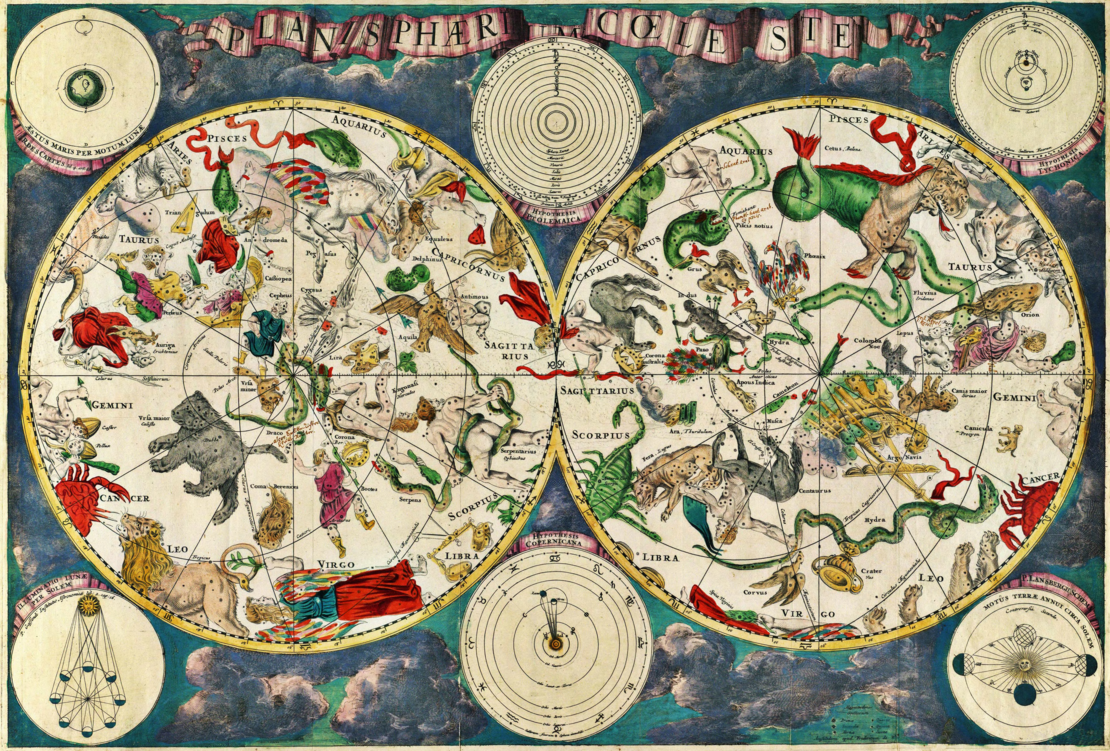
\includegraphics[height=2cm]{inputs/starchart}
      \begin{center} \only<1>{star map}\only<2>{\sout{star map} star chart}\end{center}
    \end{column}
    \begin{column}{0.3\textwidth}
      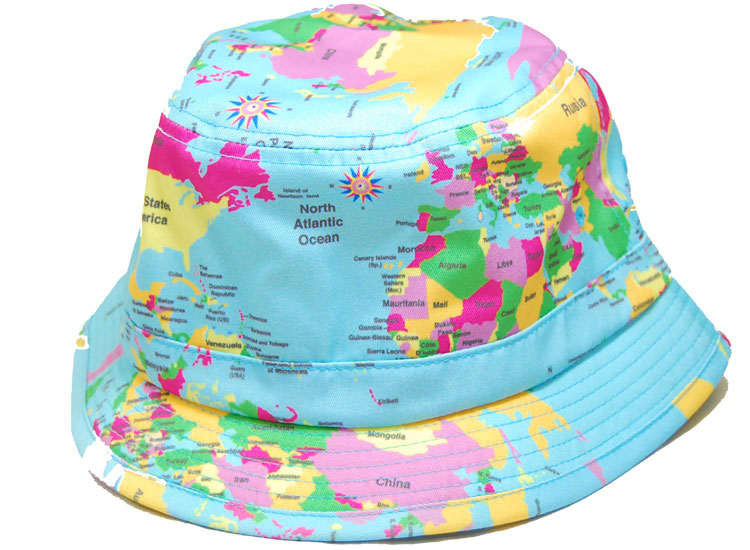
\includegraphics[height=2cm]{inputs/maphat.jpg}
      \begin{center}\only<1>{hat map}\only<2>{\sout{hat map} map hat}\end{center}
    \end{column}
  \end{columns}
\end{frame}


%%%%%%%%%%%%%%%%%%%%%%%%%%%
\begin{frame}[fragile,label=P5Lemma]{The Star Map and Hat Map}

  %% \begin{exampleblock}{}
    
  \begin{columns}
    \begin{column}{0.25\textwidth}
      
\includegraphics[height=3cm]{inputs/amnotconfus.jpg}
    \end{column}
    \begin{column}{.8\textwidth}
      \begin{itemize}
      \item[star map] 
        $^*:\Con\bB \rightarrow \Con\bA$ is
        congruence generation: %restricted to the set $\Con\bB$:
        \[\beta^* = \Cg^\bA(\beta)\qquad (\forall \, \beta \in \Con\bB)\]
        \vskip3mm
      \item[hat map]
        $\hatmap: \Con\bB \rightarrow \Con\bA$ is
      \[\widehat{\beta} =
        \{(x,y) \in A^2 \mid (ef(x), ef(y))\in \beta,
        \;\forall\, f\in  \Pol_1(\bA) \}.\]
             \note{
               It is not hard to see that $\hatmap$ maps $\Con\bB$ into $\Con\bA$.
               For example, if $(x,y) \in \widehat{\beta}$ and $g\in \Pol_1(\bA)$,
               then for all $f\in \Pol_1(\bA)$ we have $(efg(x),efg(y)) \in \beta$,
               so $(g(x),g(y))\in \widehat{\beta}$.}
      \end{itemize}
    \end{column}
  \end{columns}
  %% \end{exampleblock}
  \vskip1cm
  \visible<2>{{\small The hat map appears in McKenzie's ``Finite Forbidden Lattices''
      paper (Puebla, 1982) where he gives an alternative proof of the $P^5$ Lemma.}}

    %% \end{exampleblock}
  %% \vskip5mm{\small       Ralph McKenzie: {\it Finite forbidden lattices.} Puebla (1982).}
\end{frame}

%%%%%%%%%%%%%%%%%%%%%%%%%%%
\begin{frame}[fragile,label=P5Lemma]{Residuation lemma}
A lemma relating the three maps $\,^*\,$, $\, \resB\,$ and $\,\hatmap$.
\vskip2mm

\begin{lemma} %[D, 2011]
\label{lem:residuation-lemma}
  \begin{enumerate}[(i)]
  \item $^*: \Con\bB \rightarrow \Con\bA$ is a \defn{residuated mapping} with
    \defn{residual} $\resB$.
  \item $\resB : \Con\bA \rightarrow \Con\bB$ is a \defn{residuated mapping} with
    \defn{residual} $\hatmap$.
  \item For all $\alpha \in \Con\bA, \, \beta \in \Con\bB$,
    \[\beta = \alpha\resB \quad \Leftrightarrow  \quad 
    \beta^* \leq \alpha \leq \widehat{\beta}.\]
    In particular, 
    $\beta^*\resB = \beta = \widehat{\beta}\resB$.
  \end{enumerate}
\end{lemma}

\note{
{\small If $X$ and $Y$
  are partially ordered sets, and if 
  $f: X \rightarrow Y$ and 
  $g: Y \rightarrow X$ are order preserving maps, then TFAE:
  \begin{enumerate}[(a)]
  \item $f: X \rightarrow Y$ is a {\it residuated mapping} with {\it residual}
    $g: Y \rightarrow X$;
  \item for all $x\in X,\, y\in Y$,  $f(x) \leq y$ iff $x \leq g(y)$;
  \item $g\circ f \geq \id_X$ and $f\circ g \leq \id_Y$.
  \end{enumerate}
  So, for each $y\in Y$,  $\exists !$ maximum $x\in X$ such that $f(x) \leq y$, and the
  max is given by $g(y)$.
  Thus, {\it (i)} is equivalent to 
  \begin{equation}
    \label{eq:OAi}
    \beta^* \leq \alpha \quad \Leftrightarrow \quad \beta \leq \alpha\resB
    \quad (\forall \, \alpha \in \Con\bA,\; \forall \, \beta \in \Con\bB).
  \end{equation}
  This is easily verified, as follows:  If 
  $\beta^* \leq \alpha$ then
  $\beta = (\beta^*)\resB \leq \alpha\resB$ 
  If $\beta \leq \alpha\resB$ then 
  $\beta^* \leq (\alpha\resB)^* \leq \Cg^\bA(\alpha) = \alpha$.

Statement {\it (ii)} is equivalent to 
  \begin{equation}
    \label{eq:OAii}
    \alpha\resB\leq \beta 
    \quad \Leftrightarrow \quad 
    \alpha \leq \widehat{\beta}
    \quad (\forall \, \alpha \in \Con\bA,\; \forall \, \beta \in \Con\bB).
  \end{equation}
  This is also easy to check.  For, suppose
  $\alpha\resB\leq \beta$ and $(x,y)\in \alpha$. Then $(ef(x), ef(y)) \in \alpha$
  for all $f \in \Pol_1(\bA)$ and $(ef(x), ef(y)) \in B^2$, therefore, 
  $(ef(x), ef(y)) \in \alpha\resB \leq \beta$, so $(x,y) \in \widehat{\beta}$.
  Suppose $\alpha \leq \widehat{\beta}$ and $(x,y) \in \alpha\resB$. 
  Then $(x,y) \in \alpha \leq  \widehat{\beta}$, so 
  $(ef(x), ef(y)) \in \beta$ for all $f\in \Pol_1(\bA)$, including $f=\id_A$, so 
  $(e(x), e(y)) \in \beta$. But $(x, y) \in B^2$, so $(x, y) = (e(x), e(y)) \in
  \beta$.

  Combining~(\ref{eq:OAi}) and~(\ref{eq:OAii}), we obtain statement {\it (iii)} of the lemma.}
}
\end{frame}

%%%%%%%%%%%%%%%%%%%%%%%%%%%
\begin{frame}[fragile,label=P5Lemma]{Adjunction lemma}
New version of the lemma:
\vskip2mm
{\Large 
\[^* \quad \dashv \quad \resB \quad \dashv \quad \hatmap\]
}
That is,
\begin{lemma} %[D, 2011]
\label{lem:residuation-lemma}
  \begin{enumerate}[(i)]
  \item $^*: \Con\bB \rightarrow \Con\bA$ is \defn{left adjoint} to $\resB$.
  \item $\resB : \Con\bA \rightarrow \Con\bB$ is \defn{left adjoint} to $\hatmap$.
  \item For all $\alpha \in \Con\bA, \, \beta \in \Con\bB$,
    \[\beta = \alpha\resB \quad \Leftrightarrow  \quad 
    \beta^* \leq \alpha \leq \widehat{\beta}.\]
    In particular, 
    $\beta^*\resB = \beta = \widehat{\beta}\resB$.
  \end{enumerate}
\end{lemma}
\end{frame}

%%%%%%%%%%%%%%%%%%%%%%%%%%%
\begin{frame}[fragile,label=P5Lemma]{Proof of the $P^5$ Lemma}
  \begin{lemma}[\Palfy-\Pudlak, 1980]
The restriction mapping 
\[
\Con\bA \ni \alpha \mapsto \alpha\resB = \alpha \cap B^2 \in \Con \bB
\]
is a complete lattice epimorphism. % of $\Con\bA$ onto $\Con\bB$.
  \end{lemma}
\note{
  Our approach to proving Lemma 1, which is similar to the
  proof of McKenzie, does not reveal any information about
  the permutability of the congruences of $\bA$, unlike the more direct proof
  given by \PAP. }
\begin{newproof}
  Recall, for $f: X \to Y$ a monotone function on preorders $X$ and $Y$,\\
  if $f$ has a right (left) adjoint, then $f$ preserves all joins (meets)
  that exist in $X$.\\[5pt]
  By the lemma $\resB$ has both a left and right adjoint.
\end{newproof}
\end{frame}



































% \vskip5mm
% \visible<1->{
%   \begin{columns}
%     \begin{column}{0.2\textwidth}
%       \begin{flushright}
%         \includegraphics[height=1.2cm]{qrcodeDeMeoExpansions}
%       \end{flushright}
%     \end{column}
%     \begin{column}{0.9\textwidth}
% {\small   {\it Expansions of finite algebras and their congruence lattices} (to appear)\\
%       \urlprefix  \url{http://arXiv.org/abs/1205.1106}}
%     \end{column}
%   \end{columns}
% }










%% \visible<2->{
%%   \begin{columns}
%%     \begin{column}{0.2\textwidth}
%%       \begin{flushright}
%%         
\includegraphics[height=1.5cm]{inputs/qrcodeMcKenzie1983}
%%       \end{flushright}
%%     \end{column}
%%     \begin{column}{0.9\textwidth}
%% {\small       Ralph McKenzie: {\it Finite forbidden lattices.}\\[4pt]
%%      In: Universal algebra and lattice theory ({P}uebla, 1982),\\
%%       \emph{Lecture Notes in Math.}, vol. 1004, pp. 176--205. Springer, Berlin (1983).\\
%%   \url{http://dx.doi.org/10.1007/BFb0063438}}
%%     \end{column}
%%   \end{columns}
%% }
%%   \note{In~\cite{McKenzie:1983}, McKenzie, taking Lemma 1 as a starting point,
%%     develops the foundations of what would become tame congruence theory.}












%% \begin{columns}\begin{column}{0.2\textwidth}
%%       \begin{flushright}
\includegraphics[height=1.5cm]{inputs/qrcodeP5}\end{flushright}
%%     \end{column}\begin{column}{0.9\textwidth}
%%     {\small P{\'e}ter P{\'a}l \Palfy\ and Pavel Pudl{\'a}k: {\it Congruence lattices of finite algebras\\ and
%%         intervals in subgroup lattices of finite groups.}\\[4pt]
%%       Algebra Universalis \textbf{11}(1), 22--27 (1980).\\
%%       \url{http://dx.doi.org/10.1007/BF02483080}}
%%   \end{column}
%% \end{columns}

\begin{frame}[fragile,label=OAresults,shrink=5]{The structure of the interval $[\beta^*, \hbeta]\leq \bCon \bA$.}

\vskip2mm

  \begin{itemize}
  \item If $\beta \in \Con \bB$ is a coatom of $\bCon \bB$ with $m$ congruence classes then
        the interval $[\beta^*, \hbeta]$ in $\bCon \bA$ is $\two^{m-1}$.
  \end{itemize}

  \begin{columns}
    \begin{column}{0.3\textwidth}

      {\scalefont{.8}
        \begin{tikzpicture}[scale=.6]
          \draw[rounded corners] (-1.5,-1.5) rectangle (1.5,1.5);
          \draw[rounded corners] (.5,.5) rectangle (3.5,3.5);
          \visible<2->{\draw[rounded corners] (.5,-3.5) rectangle (3.5,-.5) (-3.5,-3.5) rectangle (-.5,-.5);}
          \draw[rounded corners] (-3.5,.5) rectangle (-.5,3.5);
          \draw[rounded corners, dotted] (-1.35,.65) rectangle (1.35,1.35);  
          \draw[rounded corners, dotted] (-1.35,-.35) rectangle (1.35,.35);
          \draw[rounded corners, dotted] (-1.35,-1.35) rectangle (1.35,-.65);

          \draw (0,-2.2) node {$B_0 $};
          %%    % B1
          \draw (-2, 4) node {$B_1$};
          \draw (-1, 1) node {$b_0$};
          \foreach \i in {0,1,2} {
            \foreach \j in {1,2} {
              \pgfmathtruncatemacro{\x}{3*\i+\j}
              \draw (-\j - 1, \i + 1) node {$b^1_\x$};
            }
          }
          \foreach \i in {1,2} {
            \foreach \j in {0} {
              \pgfmathtruncatemacro{\x}{3*\i+\j}
              \draw (-\j - 1, \i + 1) node {$b^1_\x$};
            }
          }
          \draw (0, 1) node {$b_1$};

          %%    % B2
          \draw (2, 4) node {$B_2$};
          \draw (1, 1) node {$b_2$};
          \foreach \i in {0,1,2} {
            \foreach \j in {1,2} {
              \pgfmathtruncatemacro{\x}{3*\i+(2-\j)}
              \draw (\j + 1, \i + 1) node {$b^2_\x$};
            }
          }
          \foreach \i in {1,2} {
            \foreach \j in {0} {
              \pgfmathtruncatemacro{\x}{3*\i+(2-\j)}
              \draw (\j + 1, \i + 1) node {$b^2_\x$};
            }
          }
          \foreach \j in {3,4,5} {
            \draw (\j -4, 0) node {$b_\j$};
          }

          \foreach \j in {6,7,8} {
            \draw (\j -7, -1) node {$b_\j$};
          }
          \visible<2->{
            %%    % B3
            \draw (-2, -4) node {$B_3$};

            \foreach \i in {0,1,2} {
              \foreach \j in {1,2} {
                \pgfmathtruncatemacro{\x}{3*(2-\i)+\j}
                \draw (-\j - 1, -\i - 1) node {$b^3_\x$};
              }
            }
            \foreach \i in {1,2} {
              \foreach \j in {0} {
                \pgfmathtruncatemacro{\x}{3*(2-\i)+\j}
                \draw (-\j - 1, -\i - 1) node {$b^3_\x$};
              }
            }

            %%    % B4
            \draw (2, -4) node {$B_4$};
            \foreach \i in {1,2} {
              \foreach \j in {0,1,2} {
                \pgfmathtruncatemacro{\x}{3*(2-\i)+\j}
                \draw (3-\j , -\i - 1) node {$b^3_\x$};
              }
            }
            \foreach \i in {0} {
              \foreach \j in {0,1} {
                \pgfmathtruncatemacro{\x}{3*(2-\i)+\j}
                \draw (3-\j, -\i - 1) node {$b^3_\x$};
              }
            }
          }
        \end{tikzpicture}
      }
    \end{column}
    \begin{column}{0.6\textwidth}
      \vskip2mm
      \uncover<2->{
        \emph{More generally...}
        \vskip4pt
        \begin{itemize}
        \item  Suppose $\beta \in \Con \bB$ has transversal $b_{\beta(1)}, \dots, b_{\beta(m)}$.
          \vskip10pt
        \item Denote by $T_r$ the set of intersection points in the $r$-th block of $\beta$:
          \[
          T_r
          =  \bigcup_{k=1}^K B_k \cap b_{\beta(r)}/\beta.
          \]
        \end{itemize}
      }
    \end{column}
  \end{columns}
  %% \begin{columns}
  %%   \begin{column}{0.7\textwidth}
      \visible<3->{
        %        \begin{theorem}
        \vskip-2mm
        \begin{block}{}{}
          \[   \text{Then} \quad       [\beta^*, \widehat{\beta}] 
          = 
          \{\theta \in \Eq(A) : \beta^* \subseteq \theta \subseteq \widehat{\beta} \}
          \cong \prod_{r=1}^m (\Eq |T_r|)^{m-1}.
          \]
        \end{block}
      }

  %%   \end{column}
  %% \end{columns}
\end{frame}

\begin{frame}[fragile,label=OAextension,shrink=5]{Slightly more general examples...}

  Returning to our original example, the base algebra $\bB$
  is the right regular $S_3$-set, and the nontrivial relations in $\Con \bB$ are
  \vskip-2pt
  %% \begin{align*}
  %%   \alpha &=  \pb 0, 1, 2 \pb 3, 4, 5\pb \\[4pt]
  %%   \beta &=  \pb 0, 3 \pb 1, 4 \pb 2, 5 \pb \\[3pt]
  %%   \gamma &= |0, 4| 1, 5|2, 3| \\[3pt]
  %%   \delta &= |0, 5|1, 3|2, 4| 
  %% \end{align*}
\[
    \alpha =  \pb 0, 1, 2 \pb 3, 4, 5\pb \quad
    \beta =  \pb 0, 3 \pb 1, 4 \pb 2, 5 \pb \quad
    \gamma = |0, 4| 1, 5|2, 3| \quad
    \delta = |0, 5|1, 3|2, 4| \]

    \begin{tikzpicture}[scale=.7]
      % T = \{0, 1\}
      \node (150) at (1.5,0)  [draw, circle, inner sep=1.0pt] {};
      \node (01) at (0,1)  [draw, circle, inner sep=1.0pt] {};
      \node (02) at (0,2)  [draw, circle, inner sep=1.0pt] {};
      \node (115) at (1,1.5)  [draw, circle, inner sep=1.0pt] {};
      \node (215) at (2,1.5)  [draw, circle, inner sep=1.0pt] {};
      \node (315) at (3,1.5)  [draw, circle, inner sep=1.0pt] {};
      \node (153) at (1.5,3)  [draw, circle, inner sep=1.0pt] {};
      \draw[semithick] 
      (150) to (01) to (02) to (153) to (115) to (150) to (215) to (153) to (315) to (150);
      \draw[font=\small] (1.5,-.7) node {$T = \{0,1\}$};
      \draw[font=\small] (-.2,.7) node {$\alpha^*$};
      \draw[font=\small] (-.2,2.3) node {$\widehat{\alpha}$};

      % T = \{0, 1, 2\}
      \node (650) at (6.5,0)  [draw, circle, inner sep=1.0pt] {};
      \node (51) at (5,1)  [draw, circle, inner sep=1.0pt] {};
      \node (52) at (5,2)  [draw, circle, inner sep=1.0pt] {};
      \node (4515) at (4.5,1.5)  [draw, circle, inner sep=1.0pt] {};
      \node (515) at (5,1.5)  [draw, circle, inner sep=1.0pt] {};
      \node (5515) at (5.5,1.5)  [draw, circle, inner sep=1.0pt] {};
      \node (615) at (6,1.5)  [draw, circle, inner sep=1.0pt] {};
      \node (715) at (7,1.5)  [draw, circle, inner sep=1.0pt] {};
      \node (815) at (8,1.5)  [draw, circle, inner sep=1.0pt] {};
      \node (653) at (6.5,3)  [draw, circle, inner sep=1.0pt] {};
      \draw[semithick] 
      (650) to (51) to (515) to (52) to (653) to (615) to (650) to (715) to (653) to
      (815) to (650)
      (51) to (4515) to (52) to (5515) to (51);
      \draw[font=\small] (6.5,-.7) node {$T = \{0,1,2\}$};
      \draw[font=\small] (4.8,.7) node {$\alpha^*$};
      \draw[font=\small] (4.8,2.3) node {$\widehat{\alpha}$};

      % T = \{0, 2, 3\}
      \node (bot) at (11.25,-.2)  [draw, circle, inner sep=1.0pt] {};
      \node (top) at (11.25,3.2)  [draw, circle, inner sep=1.0pt] {};
      \node (a) at (9.5,1)  [draw, circle, inner sep=1.0pt] {};
      \node (A) at (9.5,2)  [draw, circle, inner sep=1.0pt] {};
      \draw[font=\small] (9.3,.7) node {$\alpha^*$};
      \draw[font=\small] (9.3,2.3) node {$\widehat{\alpha}$};


      \node (b) at (10.5,1)  [draw, circle, inner sep=1.0pt] {};
      \node (b1) at (10,1.5)  [draw, circle, inner sep=1.0pt] {};
      \node (b2) at (11,1.5)  [draw, circle, inner sep=1.0pt] {};
      \node (B) at (10.5,2)  [draw, circle, inner sep=1.0pt] {};

      \node (c) at (12,1)  [draw, circle, inner sep=1.0pt] {};
      \node (c1) at (11.5,1.5)  [draw, circle, inner sep=1.0pt] {};
      \node (c2) at (12.5,1.5)  [draw, circle, inner sep=1.0pt] {};
      \node (C) at (12,2)  [draw, circle, inner sep=1.0pt] {};

      \node (d) at (13.2,1.5)  [draw, circle, inner sep=1.0pt] {};
      \draw[font=\small] (13.6,1.5) node {$\delta^*$};
      \draw[semithick] 
      (bot) to (a) to (A) to (top) to (B) to (b1) to (b) to (b2) to (B)
      (b) to (bot) to (c) to (c1) to (C) to (c2) to (c)
      (C) to (top) to (d) to (bot);
      \draw[font=\small] (11.25,-.8) node {$T = \{0, 2, 3\}$};

    \end{tikzpicture}

    \begin{tikzpicture}[scale=.7]
      % T = \{0, 1, 2, 3\}
      \node (bot) at (3.25,0.5)  [draw, circle, inner sep=1.0pt] {};
      \node (top) at (3.25,4.5)  [draw, circle, inner sep=1.0pt] {};

      \node (a) at (1,2)  [draw, circle, inner sep=1.0pt] {};
      \node (a1) at (.5,2.5)  [draw, circle, inner sep=1.0pt] {};
      \node (a2) at (1,2.5)  [draw, circle, inner sep=1.0pt] {};
      \node (a3) at (1.5,2.5)  [draw, circle, inner sep=1.0pt] {};
      \node (A) at (1,3)  [draw, circle, inner sep=1.0pt] {};
      \draw[font=\small] (.75,1.7) node {$\alpha^*$};
      \draw[font=\small] (.75,3.3) node {$\widehat{\alpha}$};

      \node (b) at (2.5,2)  [draw, circle, inner sep=1.0pt] {};
      \node (b1) at (2,2.5)  [draw, circle, inner sep=1.0pt] {};
      \node (b2) at (3,2.5)  [draw, circle, inner sep=1.0pt] {};
      \node (B) at (2.5,3)  [draw, circle, inner sep=1.0pt] {};

      \node (c) at (4,2)  [draw, circle, inner sep=1.0pt] {};
      \node (c1) at (3.5,2.5)  [draw, circle, inner sep=1.0pt] {};
      \node (c2) at (4.5,2.5)  [draw, circle, inner sep=1.0pt] {};
      \node (C) at (4,3)  [draw, circle, inner sep=1.0pt] {};

      \node (d) at (5.5,2)  [draw, circle, inner sep=1.0pt] {};
      \node (d1) at (5,2.5)  [draw, circle, inner sep=1.0pt] {};
      \node (d2) at (6,2.5)  [draw, circle, inner sep=1.0pt] {};
      \node (D) at (5.5,3)  [draw, circle, inner sep=1.0pt] {};

      \draw[semithick] 
      (bot) to (a) to (a1) to (A) to (a2) to (a) to (a3) to (A) to (top) to 
      (B) to (b1) to (b) to (b2) to (B)
      (b) to (bot) to (c) to (c1) to (C) to (c2) to (c)
      (C) to (top) to (D) to (d1) to (d) to (d2) to (D)
      (d) to (bot);
      \draw[font=\small] (3.25,-.2) node {$T = \{0,1,2,3\}$};

      % T = \{0, 2, 3, 5\}
      \node (Rbot) at (11.25,0.5)  [draw, circle, inner sep=1.0pt] {};
      \node (Rtop) at (11.25,4.5)  [draw, circle, inner sep=1.0pt] {};

      \node (Ra) at (9,2)  [draw, circle, inner sep=1.0pt] {};
      \node (Ra1) at (8.5,2.5)  [draw, circle, inner sep=1.0pt] {};
      \node (Ra2) at (9.5,2.5)  [draw, circle, inner sep=1.0pt] {};
      \node (RA) at (9,3)  [draw, circle, inner sep=1.0pt] {};

      \node (Rb) at (10.5,1.8)  [draw, circle, inner sep=1.0pt] {};
      \node (RB) at (10.5,3.2)  [draw, circle, inner sep=1.0pt] {};
      \draw[font=\small] (10.2,1.5) node {$\beta^*$};
      \draw[font=\small] (10.2,3.4) node {$\widehat{\beta}$};

      \node (Rc) at (12,2)  [draw, circle, inner sep=1.0pt] {};
      \node (Rc1) at (11.5,2.5)  [draw, circle, inner sep=1.0pt] {};
      \node (Rc2) at (12.5,2.5)  [draw, circle, inner sep=1.0pt] {};
      \node (RC) at (12,3)  [draw, circle, inner sep=1.0pt] {};

      \node (Rd) at (13.5,2)  [draw, circle, inner sep=1.0pt] {};
      \node (Rd1) at (13,2.5)  [draw, circle, inner sep=1.0pt] {};
      \node (Rd2) at (14,2.5)  [draw, circle, inner sep=1.0pt] {};
      \node (RD) at (13.5,3)  [draw, circle, inner sep=1.0pt] {};

      \draw[semithick] 
      (Rbot) to (Ra) to (Ra1) to (RA) to (Ra2) to (Ra) 
      (RA) to (Rtop) to (RB)
      (Rb) to (Rbot) to (Rc) to (Rc1) to (RC) to (Rc2) to (Rc)
      (RC) to (Rtop) to (RD) to (Rd1) to (Rd) to (Rd2) to (RD)
      (Rd) to (Rbot);
      \draw [semithick]  
      (Rb) to [out=140,in=-140] (RB)
      (RB) to [out=-40,in=40] (Rb);
      \draw[font=\small] (10.5,2.5) node {$L$};

      \draw[font=\small] (11.25,-.2) node {$T = \{0,2,3, 5\}$};
      \draw[font=\small] (14,.5) node {$L\cong \two^2\times\two^2$};

    \end{tikzpicture}
\end{frame}
%% Since $\beta = | 0, 3 | 2, 5 | 1, 4 |$, when $T = \{0,2,3, 5\}$, the interval
%% $[\beta^*,\widehat{\beta}]$ is 
%% %$\Eq(2)^2 \times \Eq(2)^2  = \two^2\times\two^2$.  
%% $\two^2\times\two^2$.  
%% In Figure~\ref{fig:ConOverAlgebras2}, we denote this abstractly by $L$,
%% instead of drawing all 16 points of this interval.

%% \end{example}

%% Next, consider the situation depicted in the last congruence lattice of
%% Figure~\ref{fig:ConOverAlgebras2}, where 
%% $L \cong \two^2\times\two^2$, and
%% suppose we prefer that all the other $\resB$-inverse images be trivial:
%% $
%% [\beta^*,\widehat{\beta}]\cong \two^2\times\two^2; \,%\quad 
%% \alpha^*=\widehat{\alpha}; \, %\quad
%% \gamma^*=\widehat{\gamma};\,  %\quad
%% \delta^*=\widehat{\delta}.
%% $
%% In other words, we seek a finite algebraic
%% representation of the lattice in Figure~\ref{fig:ConOverAlgebras3}.
%% \begin{figure}[h!]
%%   \centering
%%     \begin{tikzpicture}[scale=.6]
%%       \node (Rbot) at (11.25,0.5)  [draw, circle, inner sep=1.0pt] {};
%%       \node (Rtop) at (11.25,4.5)  [draw, circle, inner sep=1.0pt] {};
%%       \node (Ra) at (9.25,2.5)  [draw, circle, inner sep=1.0pt] {};
%%       \node (Rb) at (10.75,1.8)  [draw, circle, inner sep=1.0pt] {};
%%       \node (RB) at (10.75,3.2)  [draw, circle, inner sep=1.0pt] {};
%%       \node (Rc) at (12,2.5)  [draw, circle, inner sep=1.0pt] {};
%%       \node (Rd) at (13.25,2.5)  [draw, circle, inner sep=1.0pt] {};
%%       \draw[semithick] 
%%       (Rbot) to (Ra) to (Rtop) to (RB)
%%       (Rb) to (Rbot) to (Rc) to (Rtop) to (Rd) to (Rbot);
%%       \draw [semithick]  
%%       (Rb) to [out=140,in=-140] (RB)
%%       (RB) to [out=-40,in=40] (Rb);
%%       \draw[font=\small] (10.75,2.5) node {$L$};
%%     \end{tikzpicture}
%%   \caption{A lattice which motivates further expansion of the set of basic 
%%     operations in the overalgebra.}
%%   \label{fig:ConOverAlgebras3}
%% \end{figure}
%% This is easy to achieve by adding more operations in the overalgebra
%% construction described above.
%% In fact, it is possible to introduce additional operations
%% so that, if $\beta = \Cg^\bB(x,y)$, then $\theta^* = \widehat{\theta}$ for all
%% $\theta \in \Con\bB$ with $\theta \ngeq \beta$. %%   \begin{itemize}
%%   \item put stuff here...
%%   \end{itemize}
%% \end{frame}

%% \begin{frame}[fragile,label=Extensions,shrink=5]{Generalizations...}
%%   \begin{itemize}
%%   \item put stuff here...
%%   \end{itemize}
%% \end{frame}

\begin{frame}[fragile,label=Limitations,shrink=5]{Limitations}

\vskip5mm

Two limitations of the foregoing construction:
\begin{enumerate}
\item The sizes $|T_r|$ of the partition lattice factors in 
\[
[\beta^*, \widehat{\beta}] \cong \prod_{r=1}^m (\Eq |T_r|)^{m-1}
\] 
are limited by the size of the blocks of $\beta$.

\vskip3mm

\item If $\beta$ is not principal, 
$[\theta^*, \htheta]$ may be non-trivial for some $\theta \ngeq \beta$.
\end{enumerate}
\end{frame}

\begin{frame}[fragile,label=OAextension2,shrink=5]{A Generalization}
 %% \begin{columns}
 %%  \begin{column}{0.8\textwidth}

\begin{theorem}
Let $\bB = \<B, F\>$ be a finite algebra. Suppose
\[
\beta = \Cg^{\bB}((a_1, b_1), \dots, (a_{K-1},b_{K-1}))
\]
has $m$ blocks and fix $N<\infty$.

\vskip3mm

There exists an overalgebra $\<A, F_A\>$
%Then, $\beta^* = \Cg^{\bA}(\beta)$ is given by
such that the interval $\beta\resB^{-1} \leq \Con \bA$ is 
%If $\beta$ has transversal $\{a_1, c_1, c_2, \dots, c_{m-1}\}$, then
%{\small \[ 
%% \beta^* = \bigcup_{j=0}^{MK} \beta^{\bB_j} \cup 
%% \left(\bigcup_{i=0}^{MK}t_i/\beta^{\bB_i}\right)^2, \quad
%%   \widehat{\beta} = \beta^* 
%% \cup 
%% \bigcup_{i=1}^{m-1}\left(\bigcup_{\ell \in \sE} c_i^\ell/\beta^{\bB_{\ell}}\right)^2
%% \cup 
%% \bigcup_{i=1}^{m-1}\left(\bigcup_{\ell \in \sO}
%% c_i^\ell/\beta^{\bB_{\ell}}\right)^2.
%% \]}
\[
[\beta^*, \widehat{\beta}] \cong (\Eq (N))^{m-1}.
\]
Moreover, we can arrange it so that $\theta^* = \widehat{\theta}$ for all $\theta \ngeq \beta$ in $\Con \bA$.
\end{theorem}

  %% \end{column}
  %% \begin{column}{0.2\textwidth}

%% \begin{align*}
%% B_0\cap B_1 &=\{a_1\}=\{a_1^{1}\},\\
%% B_1\cap B_2 &=\{b^1_1\}=\{a_2^{2}\},\\
%% B_2\cap B_3 &=\{b^2_2\}=\{a_3^{3}\},\\
%% \vdots\\
%% B_{K-2}\cap B_{K-1} &= \{b_{K-2}^{K-2}\}=\{a_{K-1}^{K-1}\},\\
%% B_{K-1}\cap B_K = B_K\cap B_{K+1}&=\{b^{K-1}_{K-1}\}=\{b^{K}_{K-1}\}=\{b^{K+1}_{K-1}\},\\
%% B_{K+1}\cap B_{K+2}&=\{a^{K+1}_{K-1}\} =\{b^{K+2}_{K-2}\},\\
%% B_{K+2}\cap B_{K+3}&=\{a^{K+2}_{K-2}\} =\{b^{K+3}_{K-3}\},\\
%% \vdots\\
%% B_{2K-2}\cap B_{2K-1} &= \{a_{2}^{2K-2}\}=\{b_{1}^{2K-1}\},\\
%% B_{2K-1}\cap B_{2K} = B_{2K}\cap  B_{2K+1}&=\{a^{2K-1}_{1}\}=\{a^{2K}_{1}\}=\{a^{2K+1}_{1}\},\\
%% B_{2K+1}\cap B_{2K+2}&=\{b^{2K+1}_{1}\} =\{b^{2K+2}_{2}\},\\
%% B_{2K+2}\cap B_{2K+3}&=\{b^{2K+2}_{2}\} =\{b^{2K+3}_{3}\},\\
%% \vdots\\
%% B_{MK-2}\cap B_{MK-1} &= \{b_{MK-2}^{K-2}\}=\{a_{MK-1}^{K-1}\},\\
%% B_{MK-1}\cap B_{MK}&=\{b^{MK-1}_{K-1}\}=\{b^{MK}_{K-1}\}.
%% \end{align*}
%% All other intersections are empty.
%%   \end{column}
%%  \end{columns}

\vskip3mm
\uncover<2->{
{\scalefont{.7}
  \begin{tikzpicture}[scale=.52]
    % B0
    \draw (0, 3.4) node {$B$};
    \draw (0,3) ellipse (.6cm and 1.2cm);

    % B1
    \draw (1,2) node {$B_1$};
    \draw (1,2) ellipse (1.2cm and .6cm);

    % B2
    \draw (3,2) node {$B_2$};
    \draw (3,2) ellipse (1.2cm and .6cm);

   \draw[font=\Large] (5, 2) node {$\cdots$};

    \draw (7,2) node {$B_{K-2}$};
    \draw (7,2) ellipse (1.2cm and .6cm);

    \draw (9,2.2) node {$B_{K-1}$};
    \draw (9,2) ellipse (1.2cm and .6cm);

    \draw (10,.7) node {$B_{K}$};
    \draw (10,1) ellipse (.6cm and 1.2cm);

    \draw (11,2.2) node {$B_{K+1}$};
    \draw (11,2) ellipse (1.2cm and .6cm);

    \draw (13,2.2) node {$B_{K+2}$};
    \draw (13,2) ellipse (1.2cm and .6cm);


   \draw[font=\Large] (15, 2) node {$\cdots$};

    \draw (16.9,1.8) node {$B_{2K-1}$};
    \draw (17,2) ellipse (1.2cm and .6cm);

    \draw (18,3.3) node {$B_{2K}$};
    \draw (18,3) ellipse (.6cm and 1.2cm);

    \draw (19.1,1.8) node {$B_{2K+1}$};
    \draw (19,2) ellipse (1.2cm and .6cm);

   \draw[font=\Large] (21, 2) node {$\cdots$};

   \node (1) at (0,2) [fill,circle,inner sep=.6pt] {};
   \draw (0, .6) node {$a_1{=}a_1^1$};
   \draw (0, 1) to  (0,1.9);

   \node (2) at (2,2) [fill,circle,inner sep=.6pt] {};
   \draw (2, 3.3) node {$b^1_1 {=} a^2_2$};
   \draw (2, 3) to  (2,2.1);

   \node (3) at (4,2) [fill,circle,inner sep=.6pt] {};
   \draw (4, .6) node {$b^2_2 {=} a^3_3$};
   \draw (4, 1) to  (4,1.9);

   \node (4) at (6,2) [fill,circle,inner sep=.6pt] {};
   \node (5) at (8,2) [fill,circle,inner sep=.6pt] {};
  \draw (7.5, .6) node {$b^{K-2}_{K-2} {=} a^{K-1}_{K-1}$};
   \draw (8, 1) to  (8,1.9);

   \node (6) at (10,2) [fill,circle,inner sep=.6pt] {};
   \draw (10, 3.4) node {$b^{K-1}_{K-1} {=} b^{K}_{K-1}{=} b^{K+1}_{K-1}$};
   \draw (10, 3) to  (10,2.1);

   \node (7) at (12,2) [fill,circle,inner sep=.6pt] {};
   \draw (12.5, .6) node {$a^{K+1}_{K-1} {=} b^{K+1}_{K-2}$};
   \draw (12, 1.2) to  (12,1.9);

   \node (8) at (14,2) [fill,circle,inner sep=.6pt] {};

   \node (9) at (16,2) [fill,circle,inner sep=.6pt] {};
   \draw (16, 3.4) node {$b^{2K-1}_{1}$};
   \draw (16, 3) to  (16,2.1);

   \node (10) at (18,2) [fill,circle,inner sep=.6pt] {};
   \draw (18, .6) node {$a^{2K-1}_{1} {=} a^{2K}_{1}{=} a^{2K+1}_{1}$};
   \draw (18, 1) to  (18,1.9);

   \node (11) at (20,2) [fill,circle,inner sep=.6pt] {};
   \draw (20, 3.4) node {$b^{2K+1}_{1}$};
   \draw (20, 3) to  (20,2.1);
   
  \end{tikzpicture}
}
}
\end{frame}



    \end{document}


    %%%%%%%%%%%%% END DOCUMENT %%%%%%%%%%%%%%%%
